\documentclass[10pt]{beamer}


\mode<presentation> 
{
  \usetheme{Diku}
  \beamertemplatenavigationsymbolsempty
  \setbeamercovered{invisible}
%  \setbeamercovered{transparent}
}


% \usepackage[danish]{babel}
\usepackage[latin1]{inputenc}
\usepackage{times}
\usepackage[T1]{fontenc}
\usepackage[english]{babel}
\usepackage{hyperref}
\usepackage{animate}
%\usepackage{multimedia}
\usepackage{francois-preamble}
\usepackage{multirow}

\usepackage{multirow}
%\usepackage{movie15}

\newcommand{\cc}{{c\!\!,}}
\newcommand{\degr}[1]{{{#1}^\circ}}

\title{VIP: Color Image Analysis}

\author[S. Olsen] % (optional, use only with lots of authors)
{S�ren Olsen}

\institute[DIKU] % (optional, but mostly needed)
{
  Department of Computer Science\\
  University of Copenhagen
}

\date[2015-16 B1] % (optional, should be abbreviation of conference name)
% {Research Presentation, Diku 2006}


% Insert page numbers
\pagenumbering{arabic}
\setbeamertemplate{footline}{\hspace{5pt}\insertpagenumber\vspace{10pt}}


\definecolor{gold}{rgb}{0.95,0.83,0.0}
\definecolor{orange}{rgb}{0.95,0.7,0.0}
% \definecolor{backblue}{rgb}{0.93,0.94,0.99}
\definecolor{backblue}{rgb}{0.95,0.94,0.99}
\setbeamercolor*{background canvas}{bg=backblue} 



\newcommand{\myemph}[1]{{\color{blue}{#1}}}
\newcommand{\intrg}[1]{\int_{{#1}=-\infty}^\infty}
\newcommand{\intRR}{\int_{-\infty}^\infty}

\AtBeginSection[]
{
  \begin{frame}<beamer>{Outline}
    \tableofcontents[currentsection,currentsubsection]
  \end{frame}
}

\begin{document}
\maketitle




%-------------------------------------------------------------------
%   Start slides
%-------------------------------------------------------------------

\begin{frame}
\frametitle{Course evaluation}
{\Large
  {\color{blue}{The course evaluation is open until Januar 16}}
  \\[5mm]
 
Please fill out the course evaluation.  \\[4mm]
{\color{red}{It does matter !!!}}
}
\end{frame}


%-------------------------------------------------------------------
\begin{frame}
\frametitle{VIP: Color Image Analysis} 

\begin{center}
{\huge \color{red}{\bf Colors don't exist!}} \\[6mm]
\end{center}

Humans sense electro magnetic radiance with wavelength $\lambda$ 
between 400 nm and 700 nm as colored light.

$$
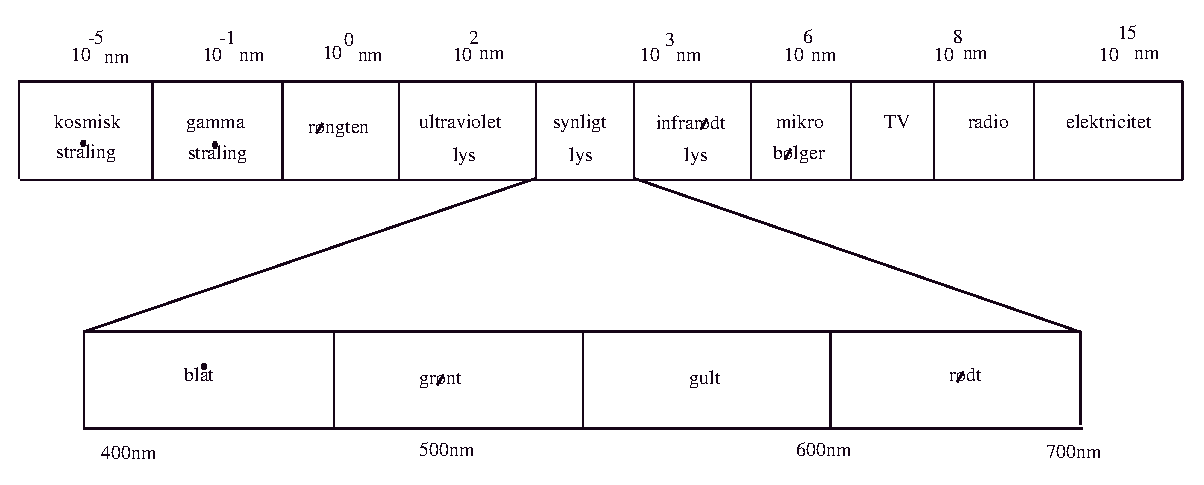
\includegraphics[width=8.0cm]{../FIGURES/elektro.eps}
$$
\end{frame}



%-------------------------------------------------------------------
\begin{frame}
\frametitle{Colors of surfaces}
$$
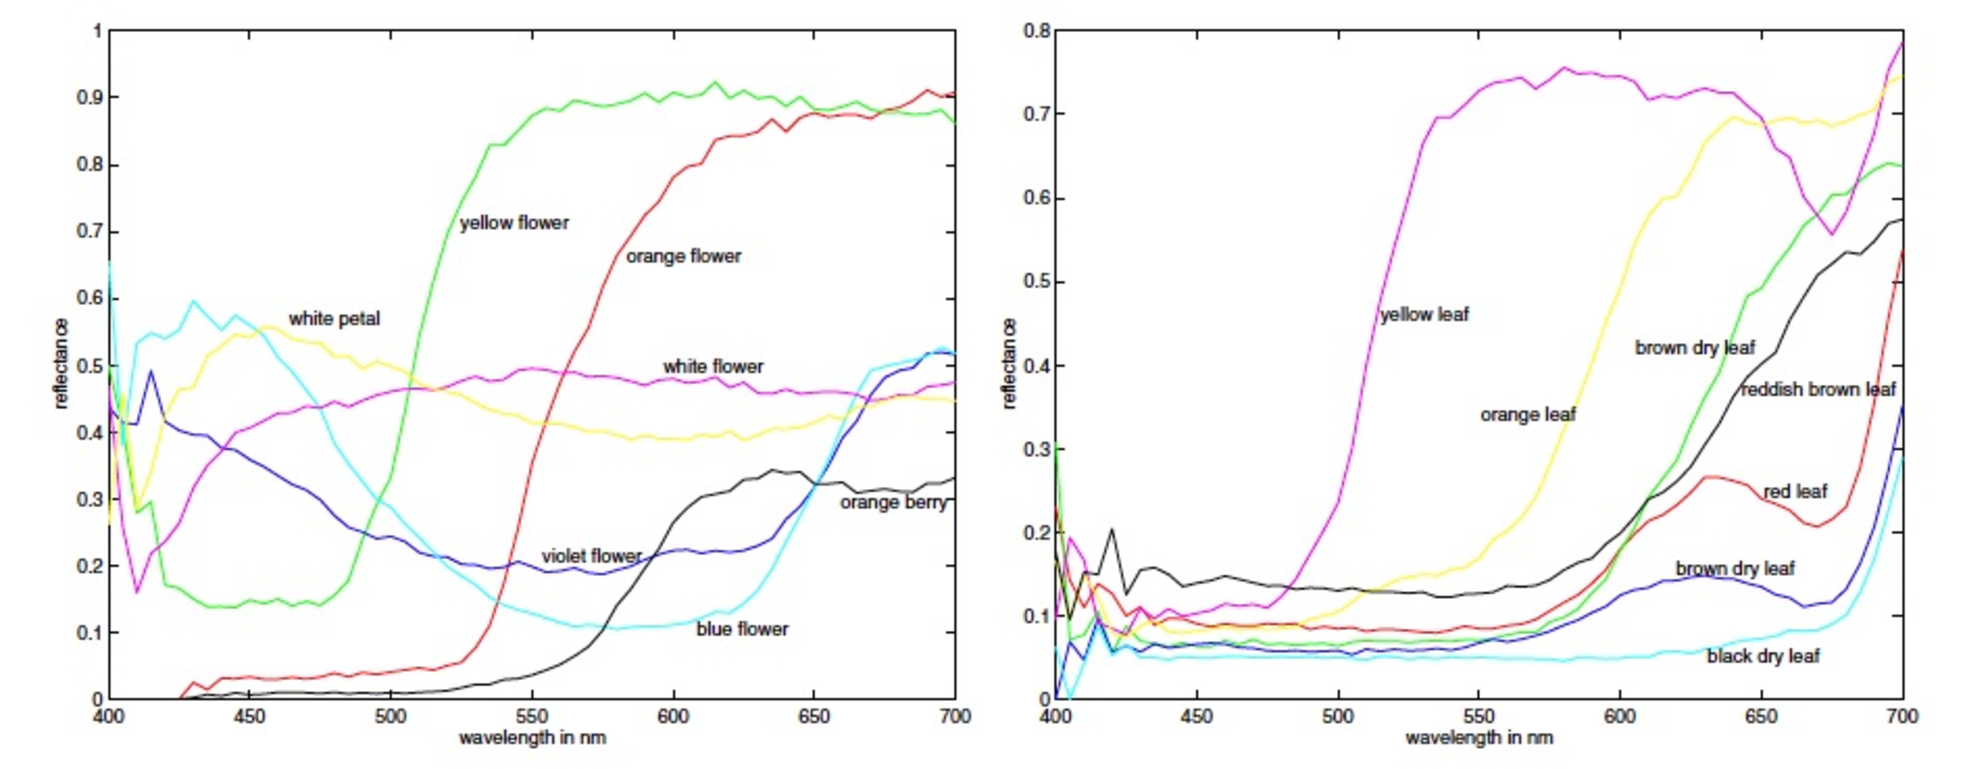
\includegraphics[width=11.0cm]{../IMAGES/SurfaceColorsFP.pdf}
$$
From Forsyth and Ponce.
\end{frame}




%-------------------------------------------------------------------
\begin{frame} 
\frametitle{Illuminant spectral power distribution}
\begin{center}
\begin{tabular}{c c}
       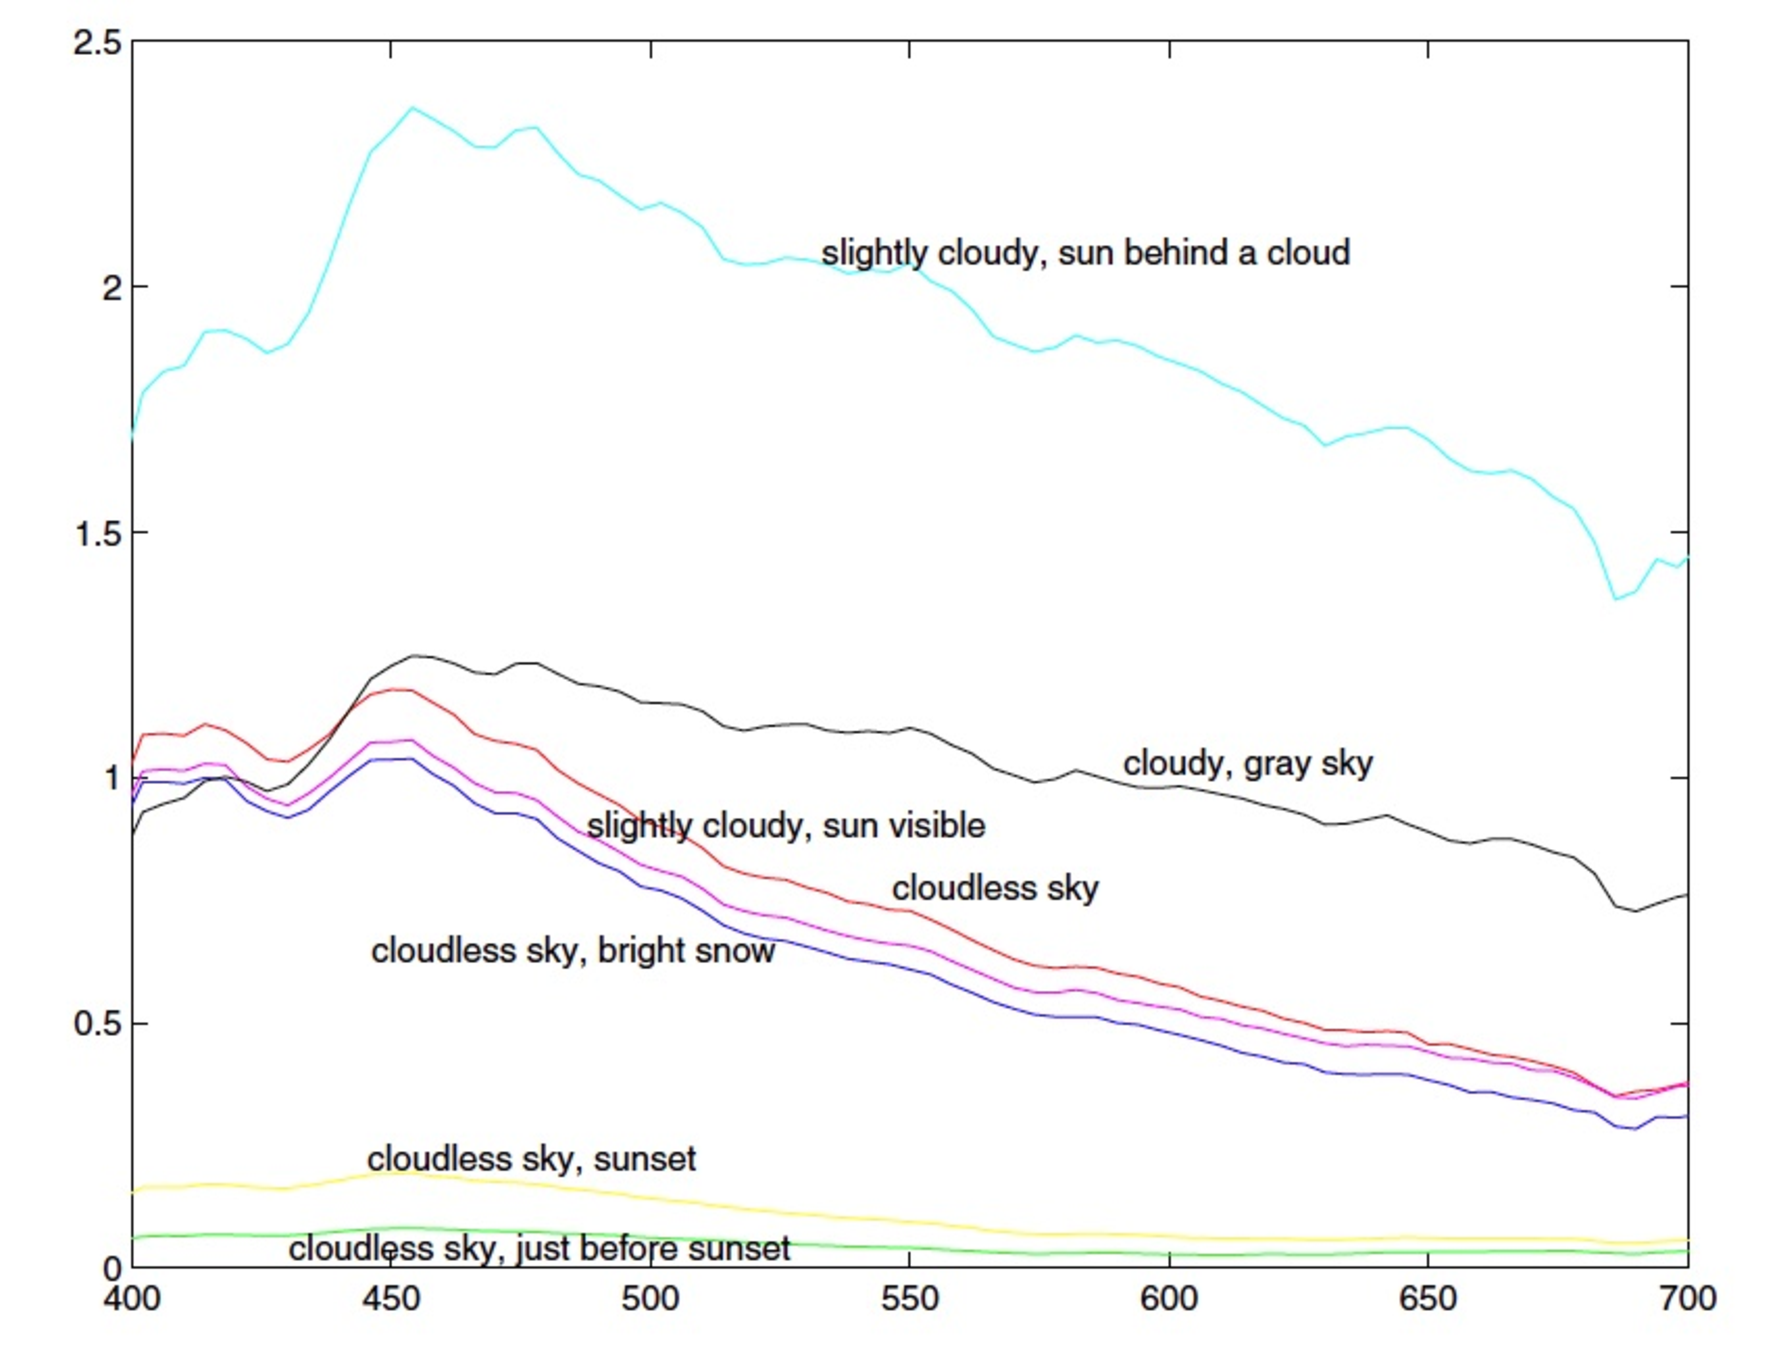
\includegraphics[width=49mm]{../IMAGES/IlluminantColor.pdf} &
       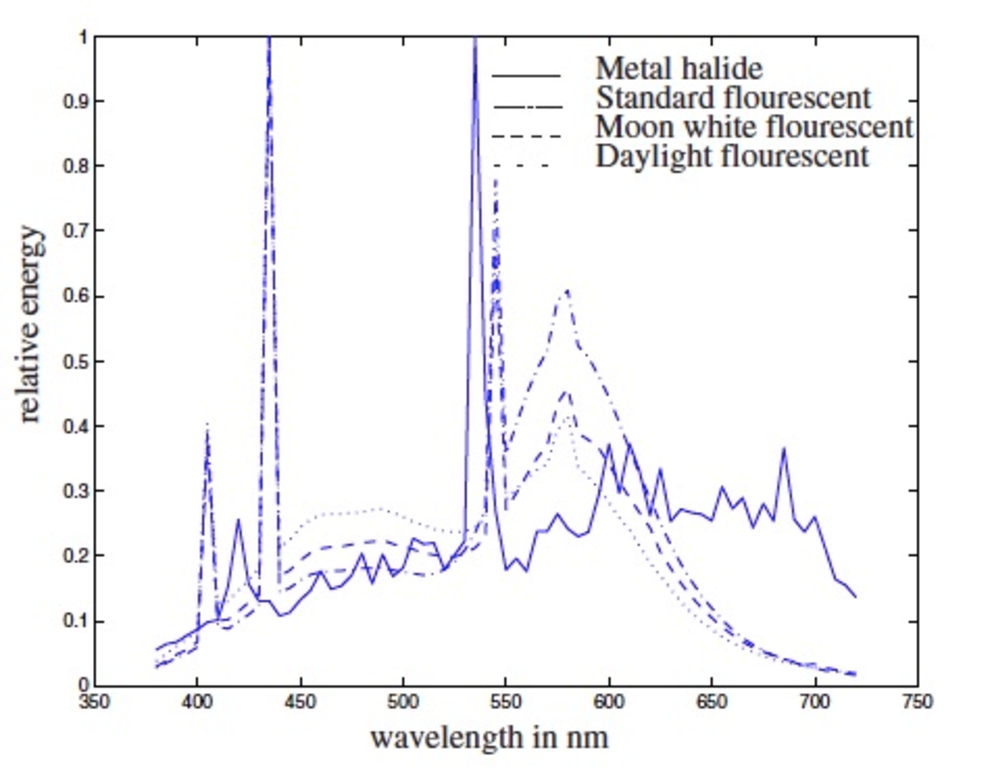
\includegraphics[width=49mm]{../IMAGES/IlluminantColor2.pdf}
\end{tabular}
\end{center}
From Forsyth and Ponce.
\end{frame}



%-------------------------------------------------------------------
\begin{frame} 
\frametitle{The temperature of light}
Electronic radiation often is modelled as emitted from a black body
that does not reflect any other light. The emitted energy distribution 
depends in a simple way of only the temperature $T$ of the body:

\begin{displaymath}
  E(\lambda) \;=\; C \; \frac{1}{\lambda^5} \;
        \frac{1}{e^{hc / k \lambda T} -1}
\end{displaymath}
where 
\begin{itemize}
\item $T$ is the temperature in Kelvin
\item $c$ is the speed of light
\item $h$ is the Planck's constant
\item $k$ is the Boltzmann's constant
\item $C$ is a constant.
\end{itemize}
\end{frame}



%-------------------------------------------------------------------
\begin{frame} 
We will later today see how the relation between energy distribution
and temperature may help in detecting and removing shadows in images.

$$
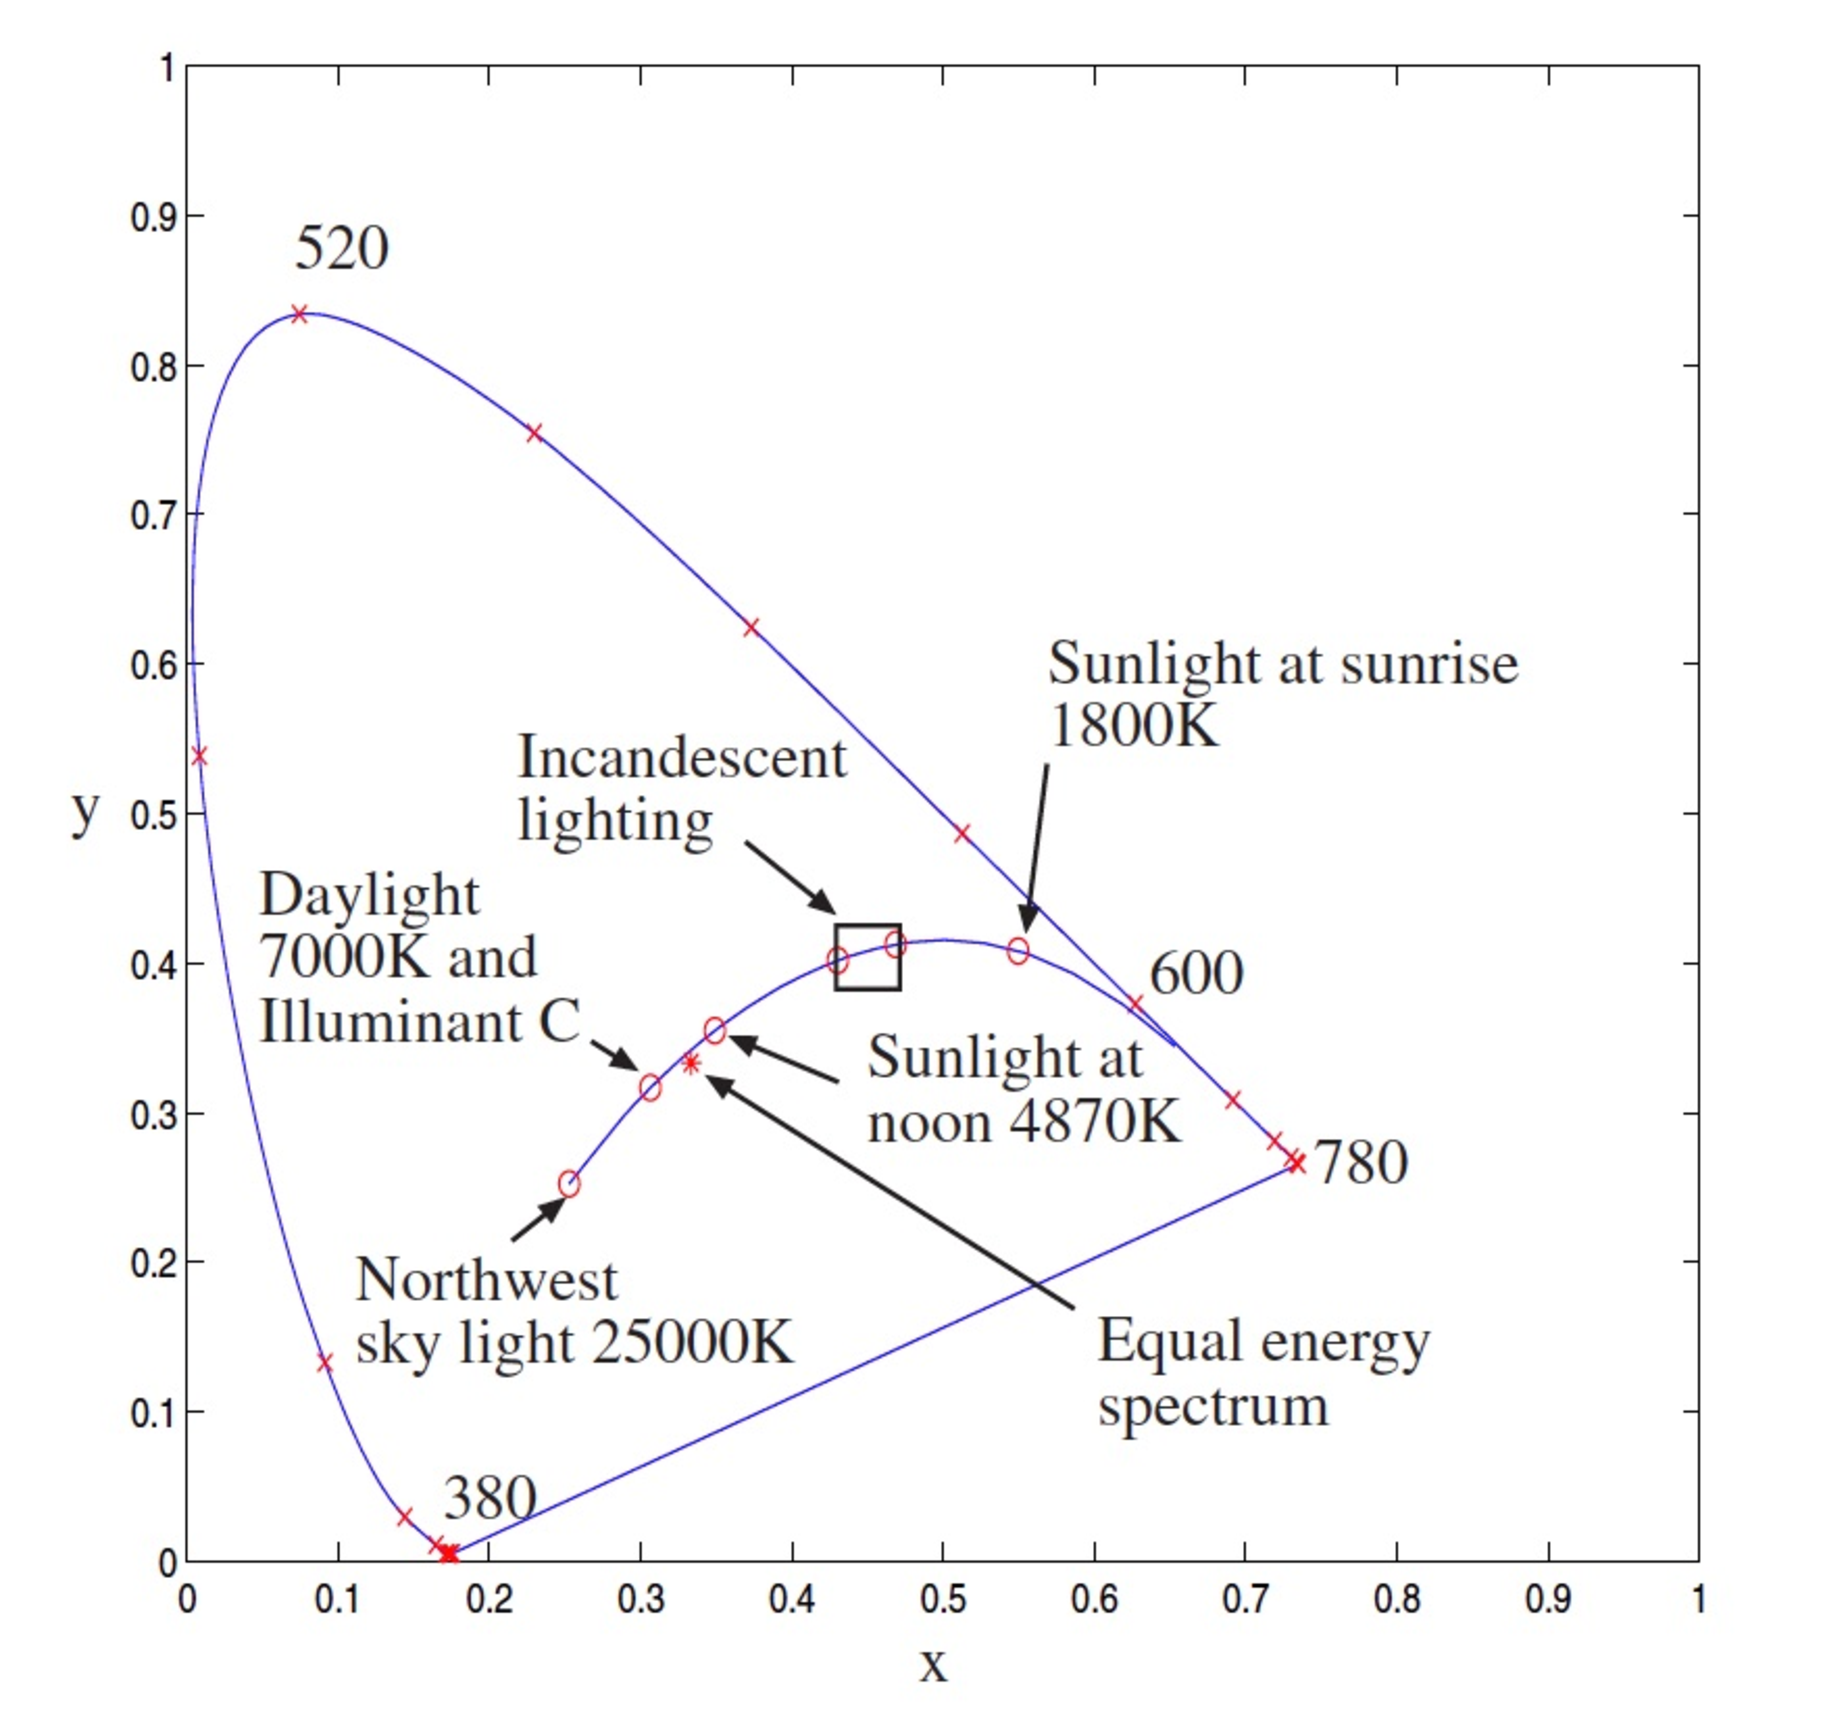
\includegraphics[width=6.5cm]{../IMAGES/GammutFP.pdf}
$$
From Forsyth and Ponce and using the CIE xy color space.
\end{frame}



%-------------------------------------------------------------------
\begin{frame} 
\frametitle{Color distribution}
$$
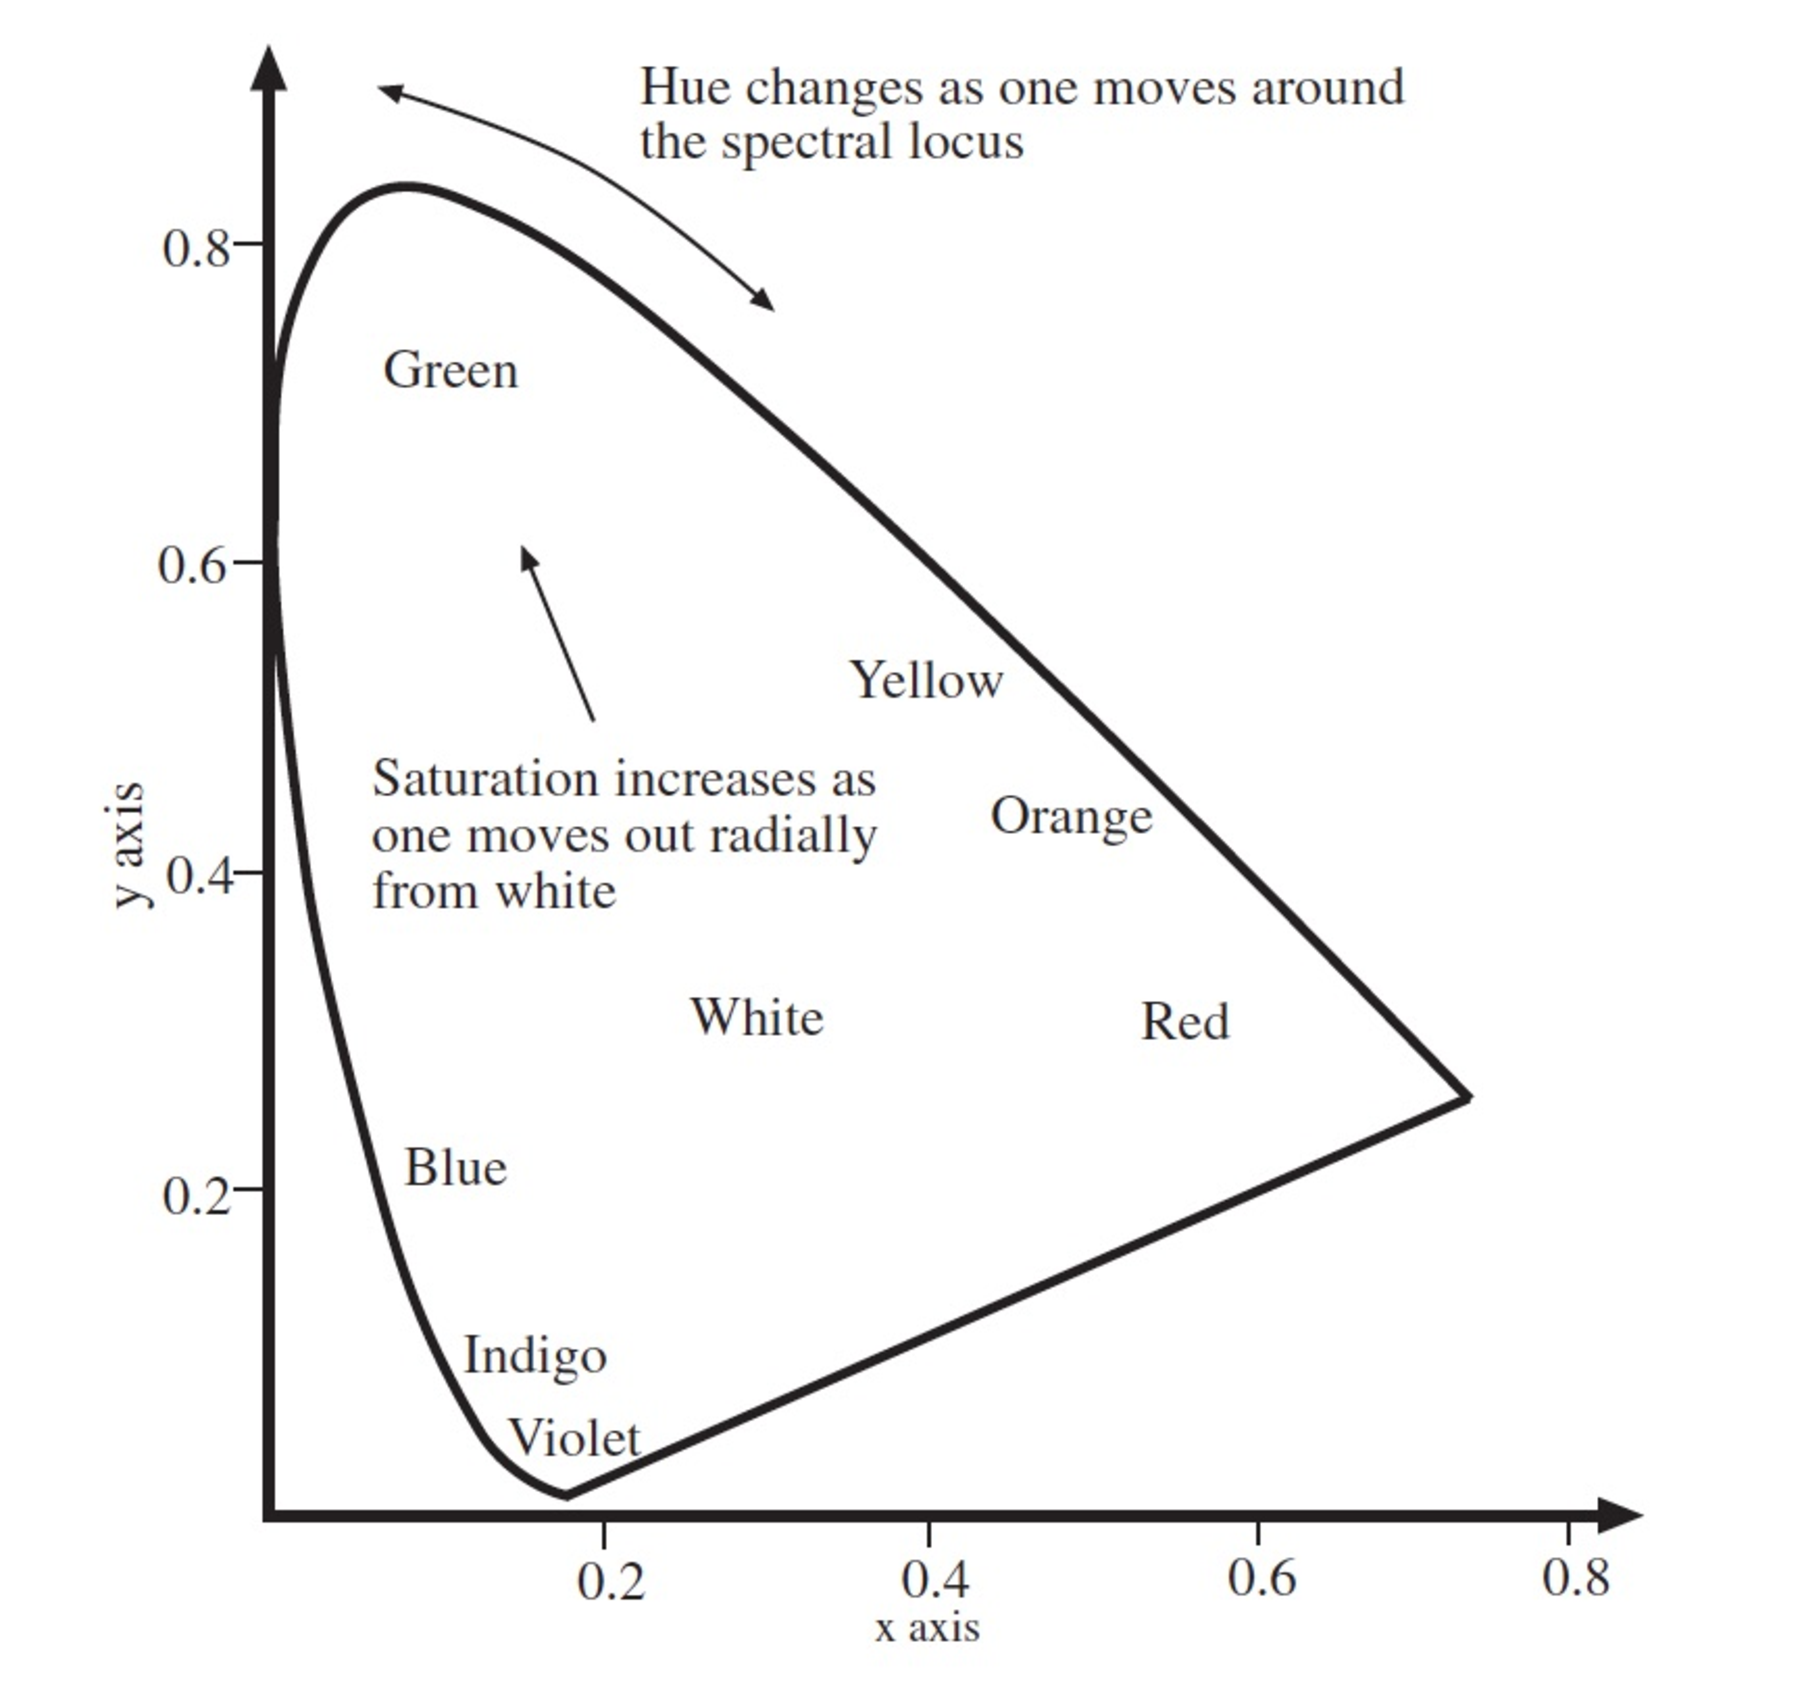
\includegraphics[width=7.0cm]{../IMAGES/ColorDistribution.pdf}
$$
From Forsyth and Ponce.

\end{frame}



%-------------------------------------------------------------------
\begin{frame} 
\frametitle{Trichromacity}
People generally agree that any (most) visible colors may be composed
by a linear combination of three different reference/primary colors (read:
R,G, and B). This is the principle of trichomacity. \\[3mm]

However, no electronic wave of any wavelength $\lambda$ may be
constructed by linear combination of waves with other
wavelengths. \\[3mm] 

Thus, there are different wavelengths that people associate with the
same color.  Also, there are colors that cannot be represented
uniquely in a linear vector space.
\end{frame}



%-------------------------------------------------------------------
\begin{frame} 
\begin{tabular}{l l}
  \begin{minipage}[t]{40mm}
    Visible light has a wavelength between 400 and 700 nm. The
    set of colors spanned by linear combination of $r$, $g$, og $b$
    is only a subset. \\[2mm]

    The triangle illustrates the gamut for a monitor. Colors outside
    the triangle cannot be shown.
  \end{minipage}
  &
  \begin{minipage}[t]{60mm}
  \vspace{-10mm}
  $$
     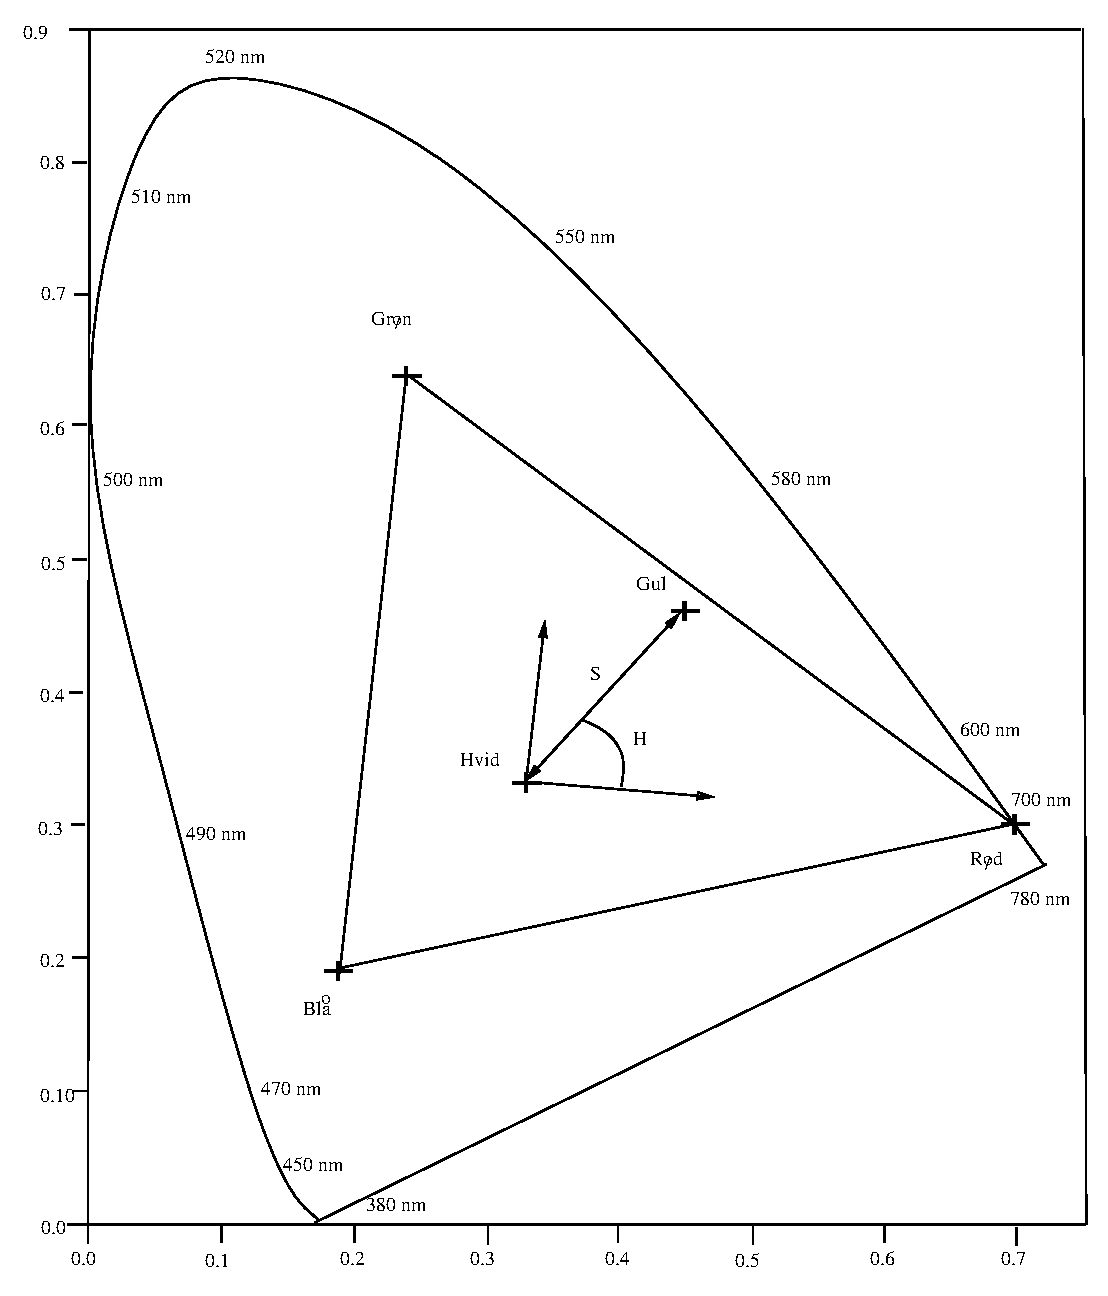
\includegraphics[width=59mm]{../FIGURES/kroma.eps}
  $$
  \end{minipage}
\end{tabular}
\end{frame}





%-------------------------------------------------------------------
\begin{frame}
By using 3 sensors, sensitive to the red, the green and the blue
part of the spectrum, it is possible to represent a subset of the
range of possible colors by one RGB-value. \\[3mm]

\begin{center}
\begin{tabular}{l r}
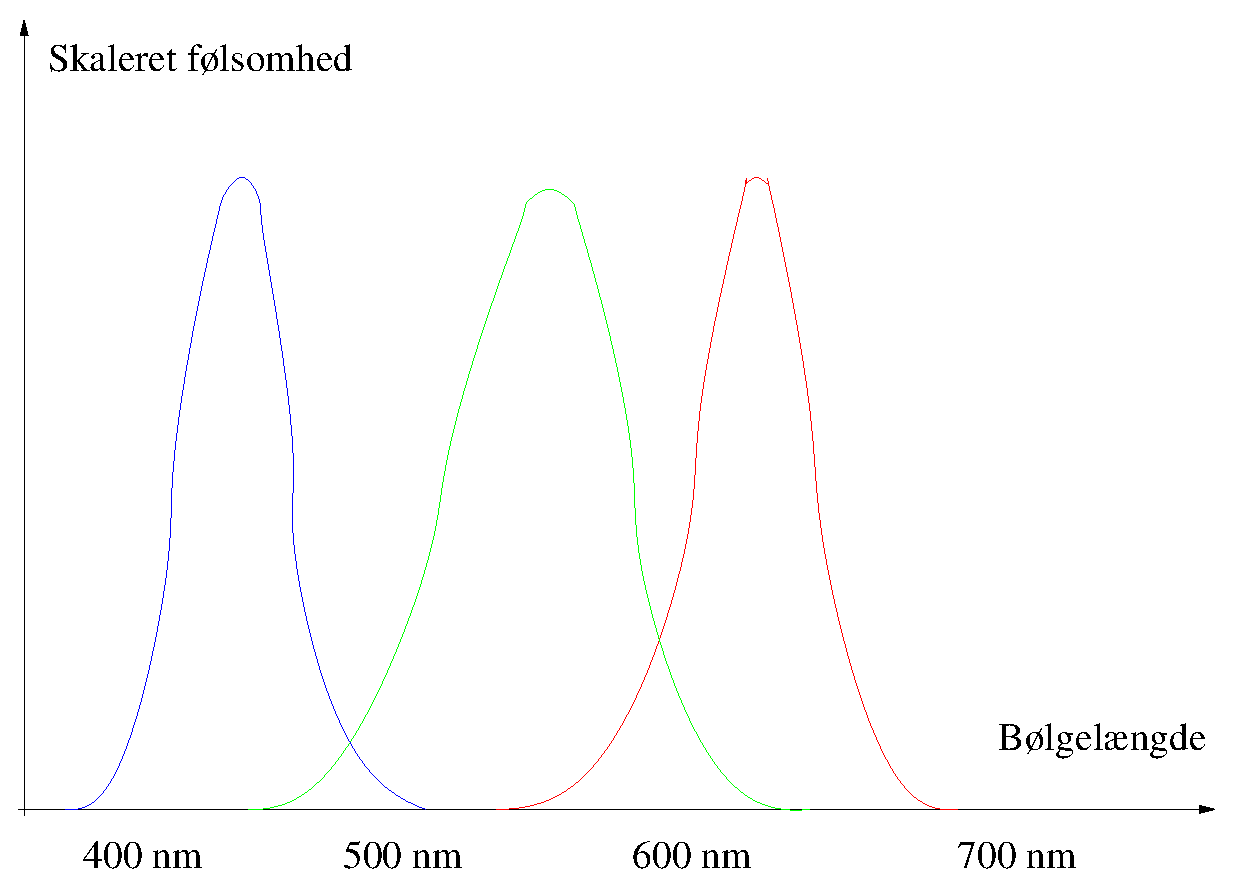
\includegraphics[width=4.5cm]{../FIGURES/spectralfilters.eps}
&
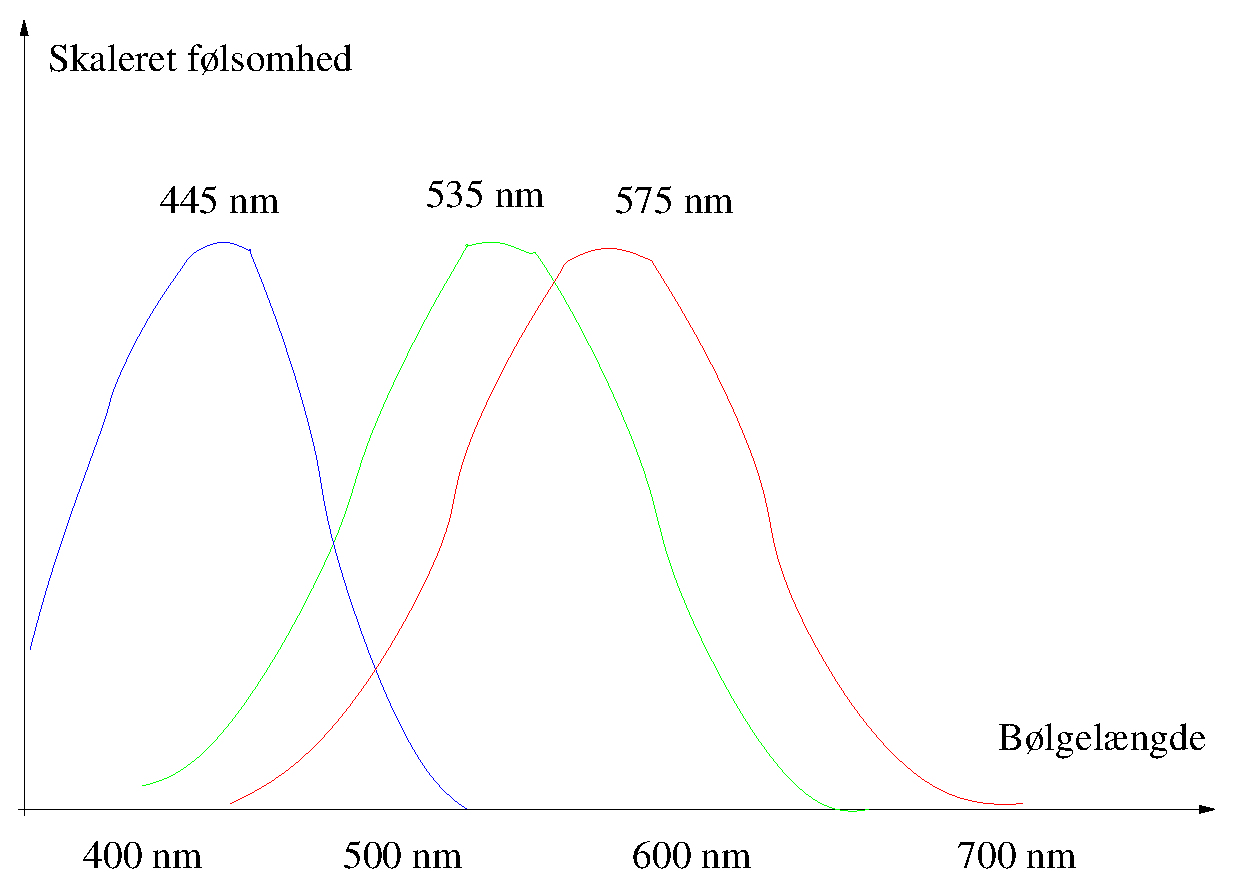
\includegraphics[width=4.5cm]{../FIGURES/humaneye.eps}
\end{tabular}
\end{center}
\vspace{3mm}

Within the human retina 3 types of cone-shaped cells exist.
These contain pigment that makes them sensitive to different
wavelengths.
\end{frame}



%-------------------------------------------------------------------
\begin{frame} 
\begin{itemize}
\item The spectral filters used by a specific camera, a color scanner
  etc. all are different.
\item The registered value depend on the spectral distribution of the
  light source $L(\lambda)$, the reflection $RF(\lambda)$ from the
  illuminated object in view, and on the specific sensor sensitivity
  curves  $f_{r/g/b}(\lambda)$.
\end{itemize}

{\small
\begin{eqnarray*}
        R & = & k_r \sum_{\lambda} L(\lambda) RF(\lambda) f_r(\lambda) \\
        G & = & k_g \sum_{\lambda} L(\lambda) RF(\lambda) f_g(\lambda) \\
        B & = & k_b \sum_{\lambda} L(\lambda) RF(\lambda) f_b(\lambda) 
\end{eqnarray*}
}
\end{frame}





%-------------------------------------------------------------------
\begin{frame} 
\frametitle{Example}

$$
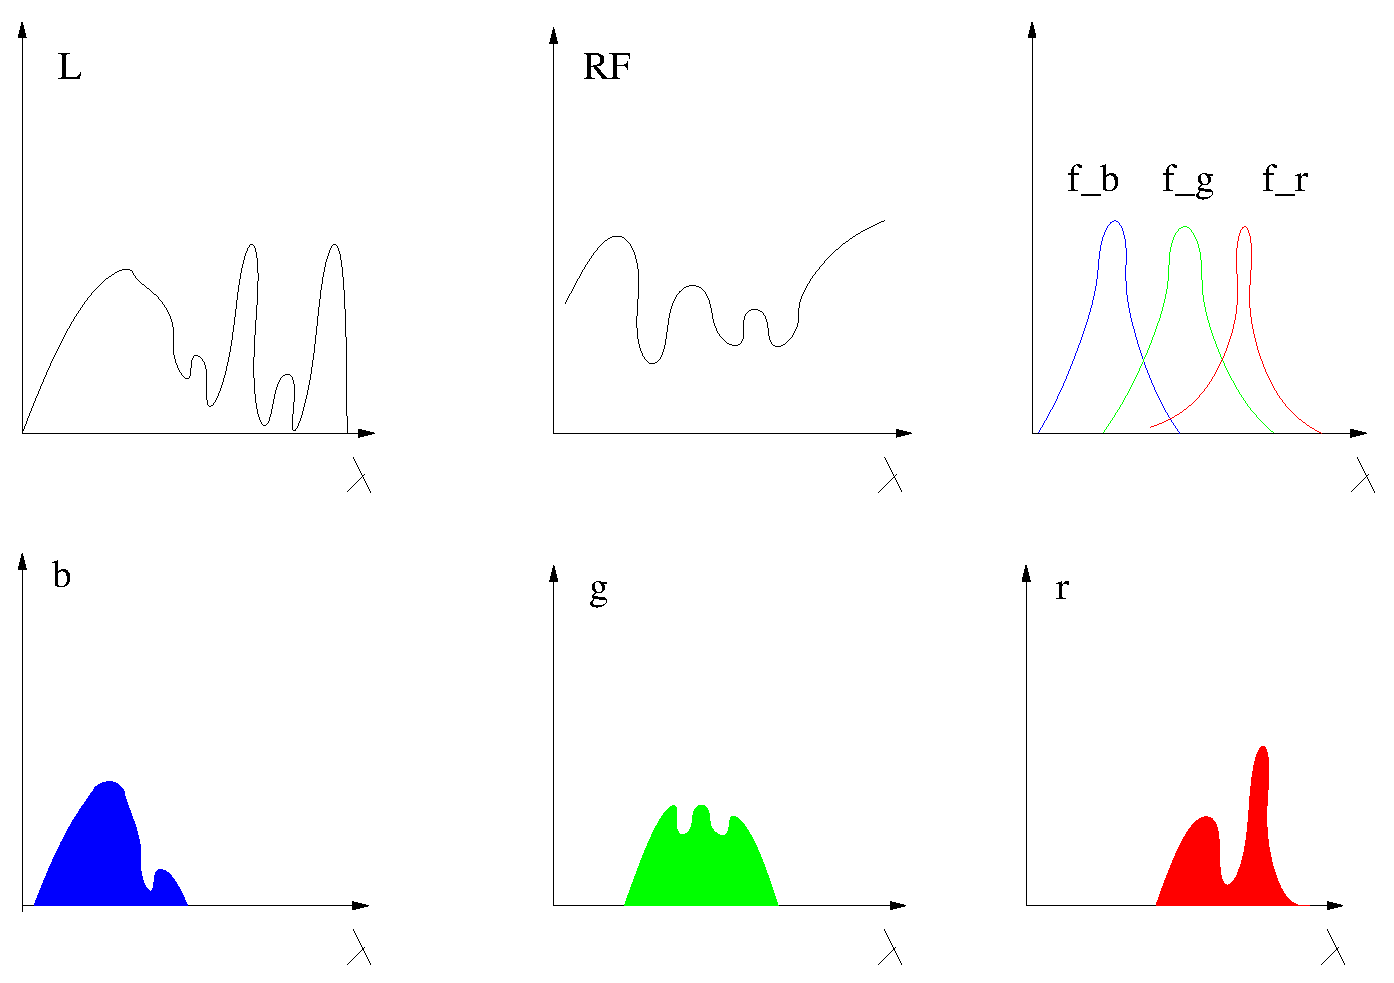
\includegraphics[width=7.8cm]{../FIGURES/spectralEX.eps}
$$
\end{frame}



%-------------------------------------------------------------------
\begin{frame} 
\frametitle{Metameterism}
\begin{itemize}
\item Two spectral distributions may be registered as having the same
  RGB-value. There is many more different spectral distributions than
  RGB values. 
\item The set of spectral distributions having the same RGB-value is
  call a {\color{red}{Metameric class}}.
\item When a color is reproduced a representative for the metameric
  class must be selected. Different monitors and printers selects
  different representatives.
\end{itemize}
\end{frame}


%-------------------------------------------------------------------
\begin{frame}
% \frametitle{Kromaticitet 1}

$$
\includegraphics[viewport=60 100 550 600,clip,width=7.4cm]{../FIGURES/fig2-12.eps}
$$
\end{frame}


%-------------------------------------------------------------------
\begin{frame} 
\frametitle{Farvesystemer}
\begin{itemize}
\item R, G, og B are called {\color{red} primary colors}. 
\item $(r,g,b)$ = $(R/I, G/I, B/I) \;\;$ are called {\color{red} the 
          trichromatic coefficients}.  $I = R+G+B$ is called the 
        {\em Intensity}. Notice: $b = 1 - r - g$. 
\item A lot of other color coordinate systems exist:\\
          CMY = (1-r, 1-g, 1-b) are (together with black K) used in
          printers. 
\item For broadcast and video  {\color{red} YIQ} (in America) and
  {\color{red} YUV} (in Europe) are used.  
\item In JPEG image coding {\color{red} $YC_bC_r$} is dominating.
\item Within graphic production the {\color{red} CIE Lab} system is used.
\item For Computer Vision the {\color{red} HSV}-system often is
  appropriate. 
\end{itemize}
$$

\includegraphics[width=3.0cm]{../FIGURES/kromim.jpg}
$$
Plot of $(r, \;g, \;1-r-g)$:
\end{frame}



%-------------------------------------------------------------------
\begin{frame} 
\frametitle{YIQ, YUV and YCbCr}
In all 3 transforms the  {\color{red}{luminance}} Y is defined by 
$ Y = 0.299 R + 0.587 G + 0.114 B$.  All 3 transforms are linear:\\[3mm]

\begin{eqnarray*}
  I = 0.74 (R - Y) \;-\; 0.27 (B - Y) \\
  Q = 0.48 (R - Y) \;+\; 0.41 (B - Y) 
\end{eqnarray*}

\begin{eqnarray*}
  U = 0.493 (B - Y) \\
  V = 0.877 (R - Y)
\end{eqnarray*} 

\begin{displaymath}
  \left [ \begin{array}{c} 
      Y \\ C_b \\ C_r \\ 
    \end{array} \right ] 
  \;\;\;=\;\;\;
  \left [ \begin{array}{r r r} 
      0.299 &  0.587 &  0.114  \\ 
      -0.169 & -0.331 &  0.5  \\ 
      0.5 & -0.419 & -0.081  \\ 
    \end{array} \right ] 
  \;\;
  \left [ \begin{array}{c} 
      R \\ G \\ B \\ 
    \end{array} \right ] 
\end{displaymath}

\end{frame}



%-------------------------------------------------------------------
\begin{frame} 
\frametitle{HSV}

\begin{tabular}{l l}
  \begin{minipage}[t]{40mm}
  $$
     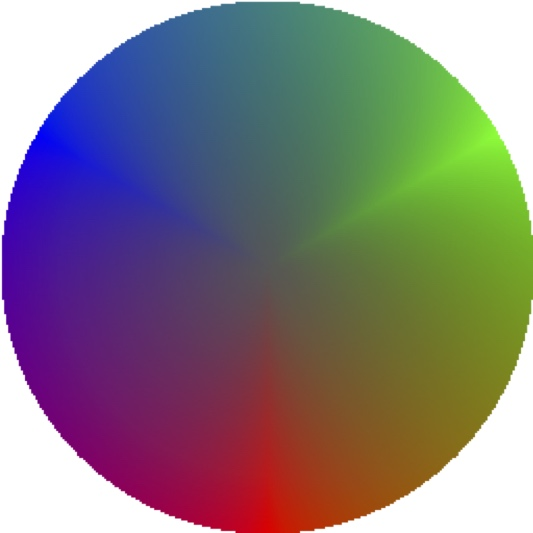
\includegraphics[width=40mm]{../FIGURES/Cim.jpg}
  $$
  \end{minipage}
  &
  \begin{minipage}[t]{40mm}
  \vspace{-10mm}
  $$
     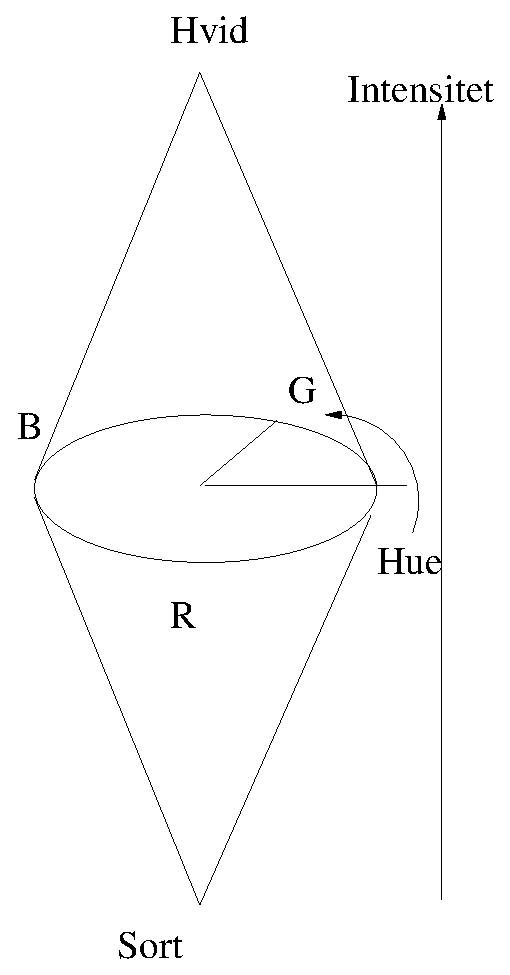
\includegraphics[width=40mm]{../FIGURES/hsvfig.eps}
  $$
  \end{minipage}
\end{tabular}
\end{frame}




%-------------------------------------------------------------------
\begin{frame} 
\frametitle{RGB2HSV}
Let
\begin{displaymath}
 \theta \;=\; \tan^{-1} \left \{
     \frac{(R - G) + (R - B)}
         {\sqrt{3} (G-B)}
\right \}
\end{displaymath}
Then {\color{red}{Hue}} H is defined by:
\begin{displaymath}
 H \;=\; \left \{
      \begin{array}{l l}
           \theta & \mbox{if B $\leq$ G} \\
           360 - \theta & \mbox{if B > G}
       \end{array} \right.
\end{displaymath}
The {\color{red}{Intensity}} is: $I = \frac{1}{3}( R + G + B)$ and
the {\color{red}{saturation}} S is defined by:
\begin{displaymath}
  S \;=\; 1 \;-\; \frac{3}{R + G + B} 
              \left [ \min \left \{ R, G, B \right \}\right ]
              \;=\; 1 \;-\ \frac{\min \left \{ R, G, B \right \}}{I}               
\end{displaymath}
Please notice that H is discontinuous at 0\\[2mm]

\end{frame}



%-------------------------------------------------------------------
\begin{frame} [fragile]
\frametitle{Why HSV}
Often we want to detect objects of specific colors in situations with
varying illumination and viewing direction.  When these factor change
the RGB-values may change significantly. Often the hue is less
sensitive.  
\medskip 

In most other transform the color is represented in 2D. In computer
Vision we are rarely interested in the saturation, so here the (used)
color  information essentially is 1D. This makes computation,
e.g. thresholding, easier. 

\end{frame}



%-------------------------------------------------------------------
\begin{frame} [fragile]
\frametitle{Example: Detection of colored object 1}
If we want to detect a green object, first notice that the color geen
has a hue value about 0.33 (on a scale from 0 to 1). Thus:
\begin{verbatim}
    green = (abs(h - 0.33) < T)
\end{verbatim}
where \texttt{T} is a user specified parameter, e.g. 0.15, defining the
width of acceptable (green) colors.\\[3mm]

In some situations, depending on the white balancing of the camera,
cloudy white may actually be greenish.  To avoid this we may:
{\small
\begin{verbatim}
    mygreen = (abs(h - 0.33) < T1) & (v < T2) & (s > T3)
\end{verbatim}
}
In this case \texttt {mygreen} will be a saturated green color.
\end{frame}



%-------------------------------------------------------------------
\begin{frame} 
% \frametitle{Eksempel}

$$
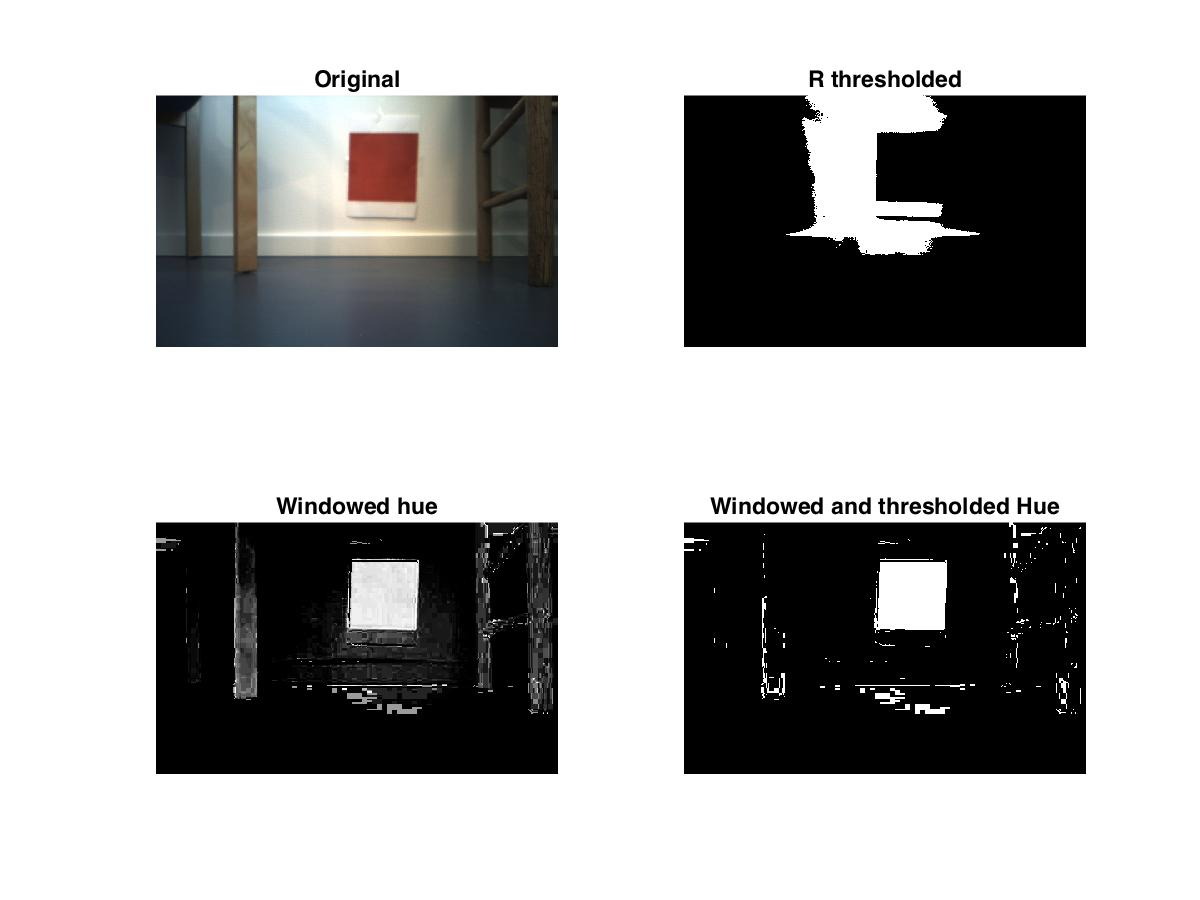
\includegraphics[width=10.0cm]{../FIGURES/Boxdetection.jpg}
$$

{\small Simple thresholding of R does not work. Use of Hue is much better.} 
\end{frame}



%-------------------------------------------------------------------
\begin{frame} 
\frametitle{Example: White balancing}
If something white is imaged as having another color, then the white
balancing is wrong and may be corrected by scaling each of the color
channels appropriately. \\[3mm]
 
First find a robust estimate of the colors having largest and smallest
intensities. Then compute a unit vector $(a,b,c)$ pointing in this
direction and scale the RGB-channels with $(\frac{1}{a},\frac{1}{b},\frac{1}{c})$
Finally, normalize to make alle values fit into $[0:1]$. \\[2mm]

\begin{center}
\begin{tabular}{c c c}
       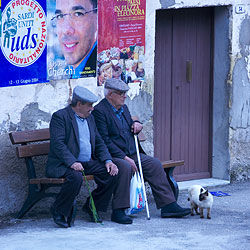
\includegraphics[width=42mm]{../IMAGES/wb_sardmen-incorrect.jpg}   
      & \hspace{1mm} &
       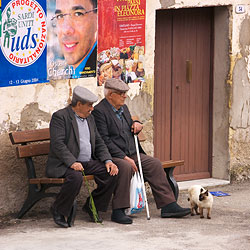
\includegraphics[width=42mm]{../IMAGES/wb_sardmen-correct.jpg}  
\end{tabular}
\end{center}
\end{frame}



%-------------------------------------------------------------------
\begin{frame} 
\frametitle{Example: Undoing automatic white balancing}
Auto white balancing may create greyish images if the scene has no
objects of e.g. the color blue.  The camera incorrectly will crank up
the sensitivity of the blue channel making the image greyish. \\[3mm]

To undo, we do like in white balancing, but instead of adjusting to a
the maximum vector $(1,1,1)$ we use the vector $(1, 1.0, 0.7)$
reflecting that the images show yellow and green colors and very little
blue.\\[2mm]

\begin{center}
\begin{tabular}{c c c}
       \includegraphics[width=49mm]{../IMAGES/IMG_0495.JPG}   
      & \hspace{1mm} &
       \includegraphics[width=52mm]{../IMAGES/ColorCorrected.png}   
\end{tabular}
\end{center}


\end{frame}



%-------------------------------------------------------------------
\begin{frame} 
\frametitle{Example: Uneven illumination}
At low sun hight angle the illuminated straw is located oposite to the
sun azimutal angle. Towards the sun, the unlit cereals is is sight. In a
HSV-representation the effect is mostly visible in S and V.
 
\begin{center}
\begin{tabular}{c c c}
       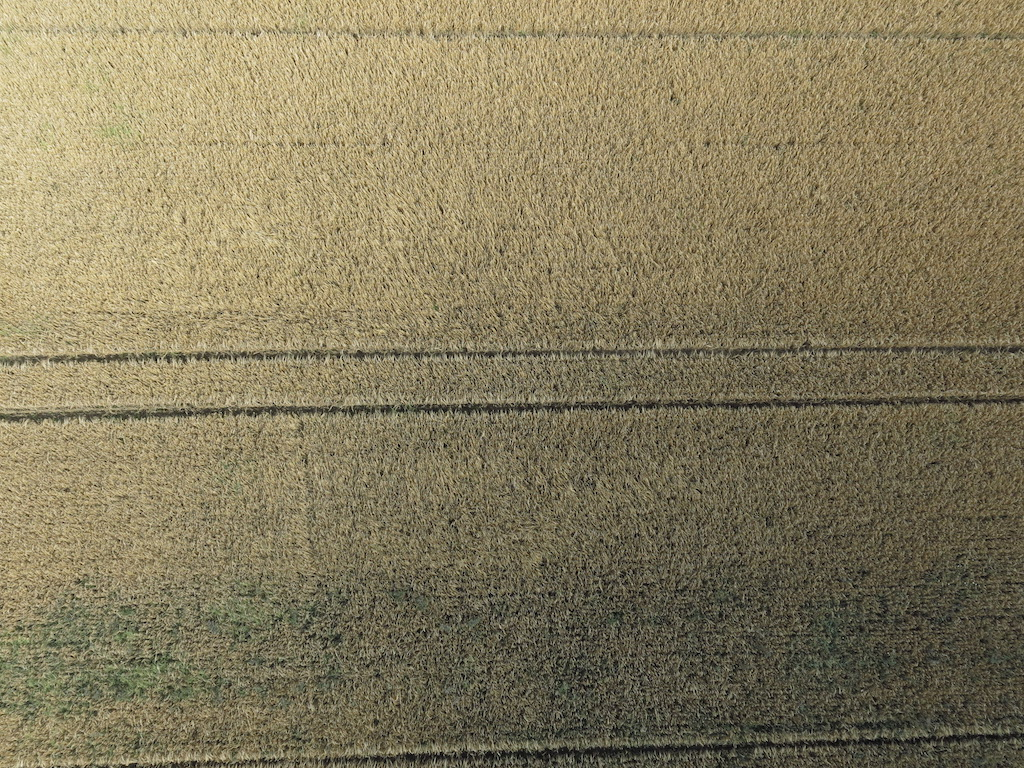
\includegraphics[width=48mm]{../IMAGES/reduced_IMG_0484.JPG}   
      & \hspace{1mm} &
       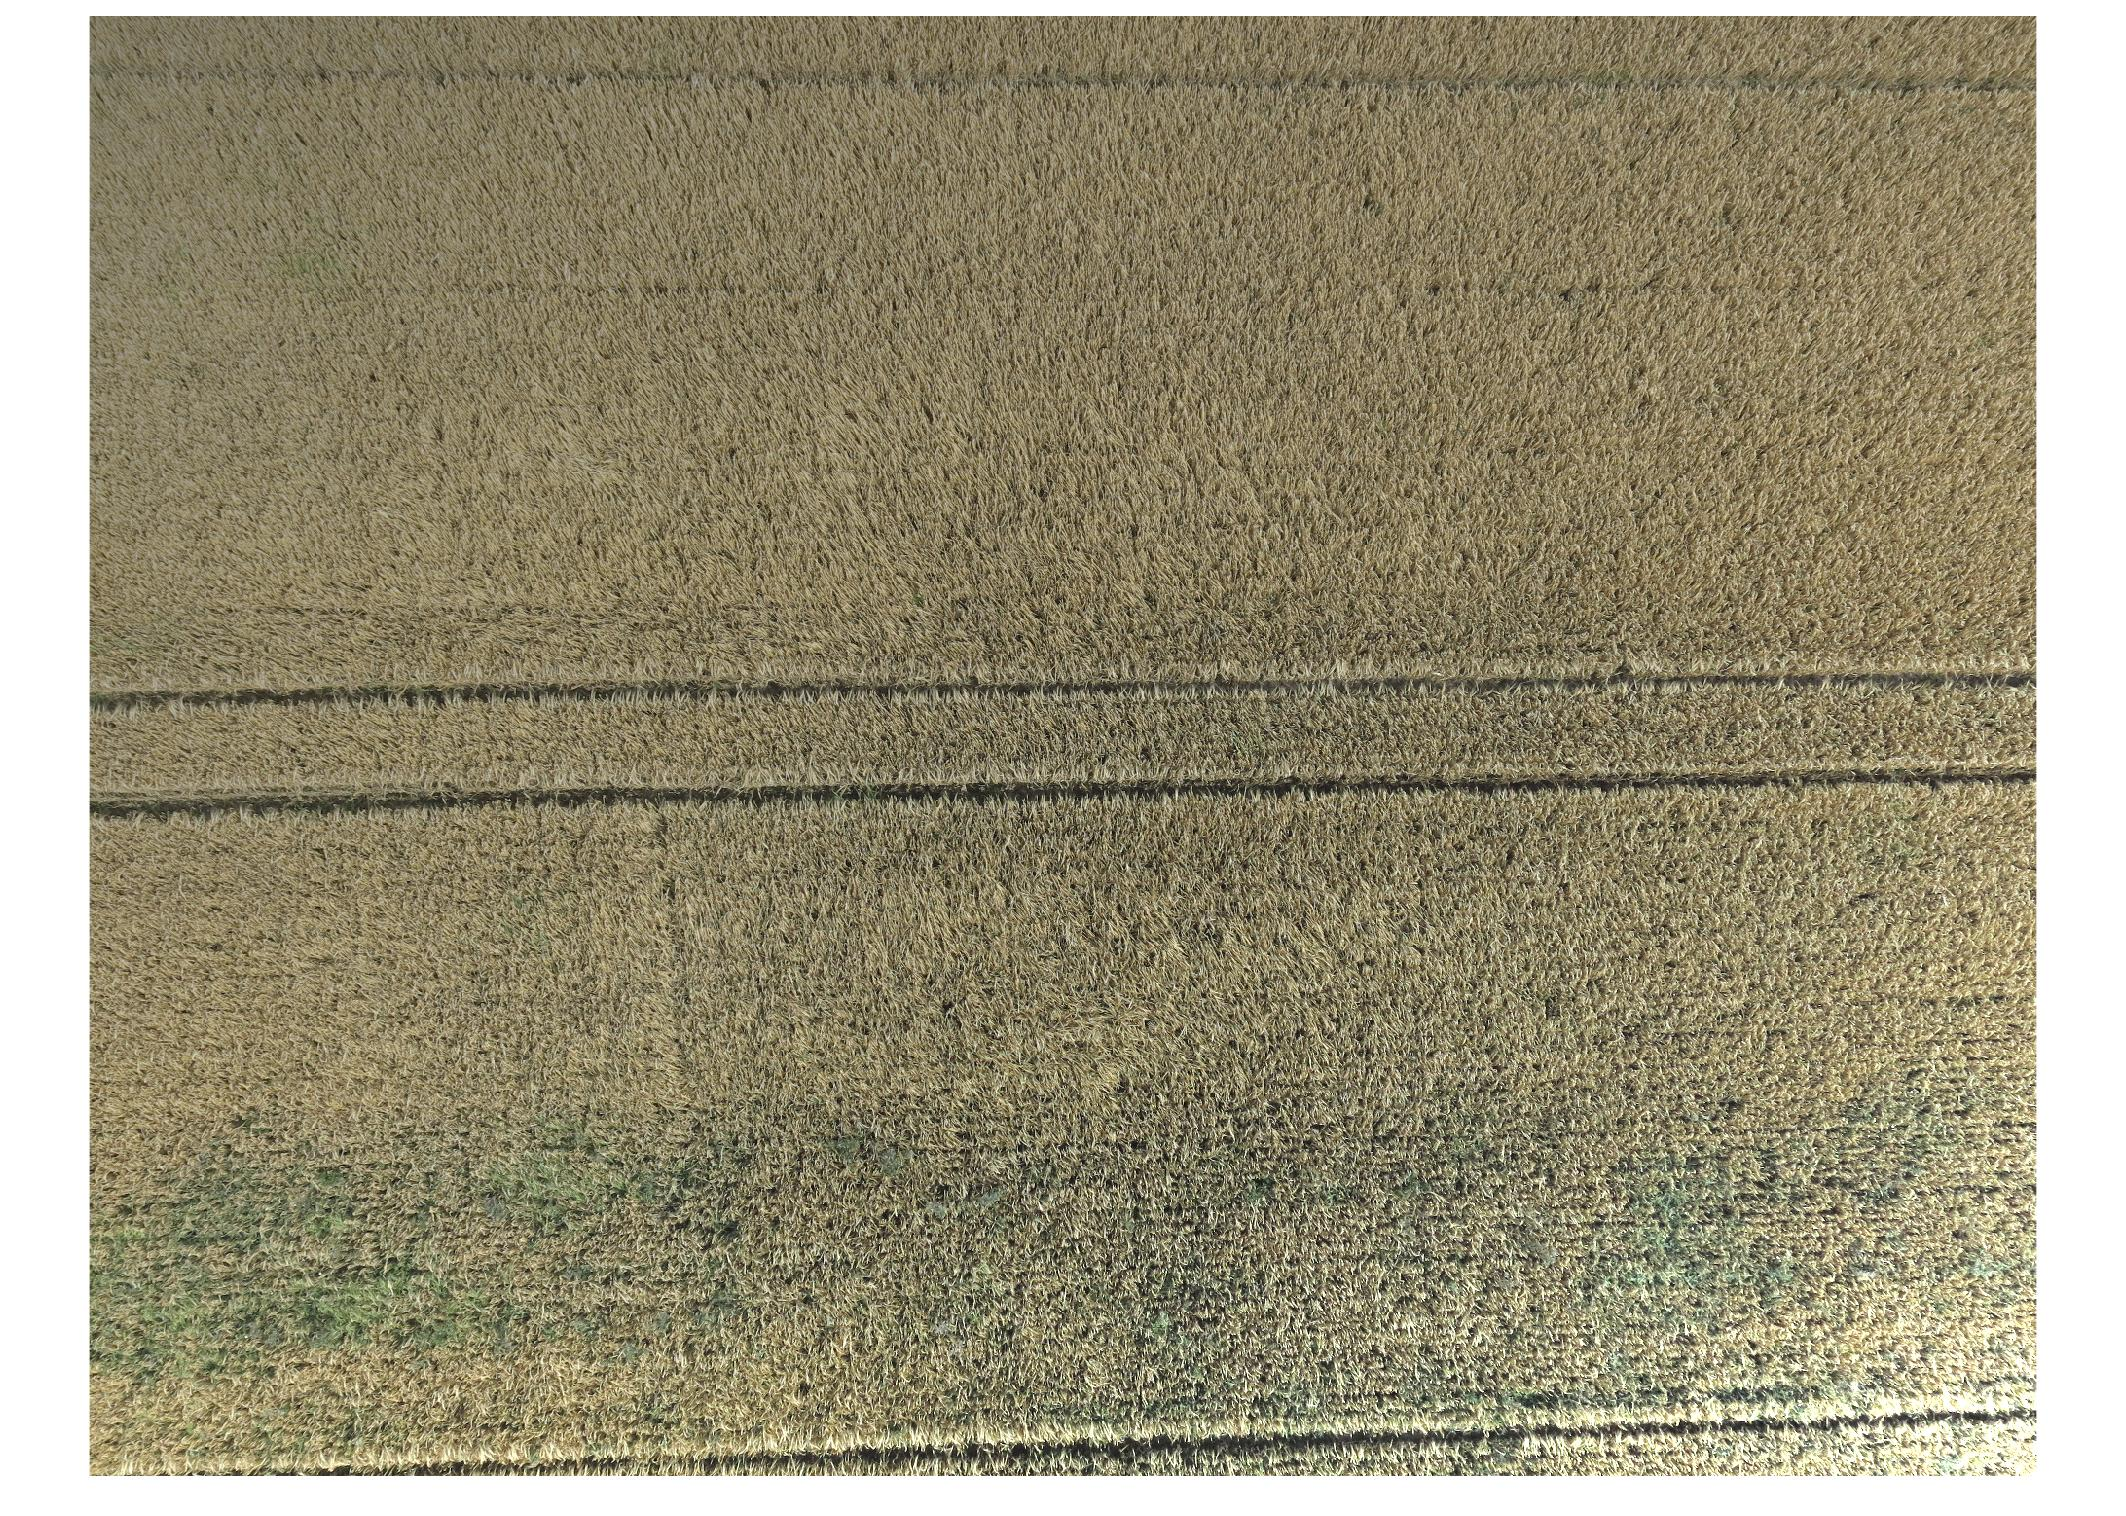
\includegraphics[width=52mm]{../IMAGES/opret0484.jpg}  
\end{tabular}
\end{center}
Both components are compensated by fitting a plane to the local
averages of saturation and value.

{\tiny
\begin{displaymath}
  S(x,y) \; \longrightarrow \;
  \frac{\bar{S}}{a_s + b_s x + c_s y} \; S(x,y)
 \hspace{6mm} \mbox{and} \hspace{6mm}
  V(x,y) \; \longrightarrow \;
  \frac{\bar{V}}{a_v + b_v x + c_v y} \; V(x,y)
\end{displaymath}
}
\end{frame}



%-------------------------------------------------------------------
\begin{frame} 
% reshape this slide using a two-column format 
\frametitle{Example: Color boosting}
When object detection is based on color information, Hue information
alone may be used.  If not, saturated colors are usually preferred.  To
increase saturation this may be nonlinearly increased:

\begin{center}
\begin{tabular}{c c c}
       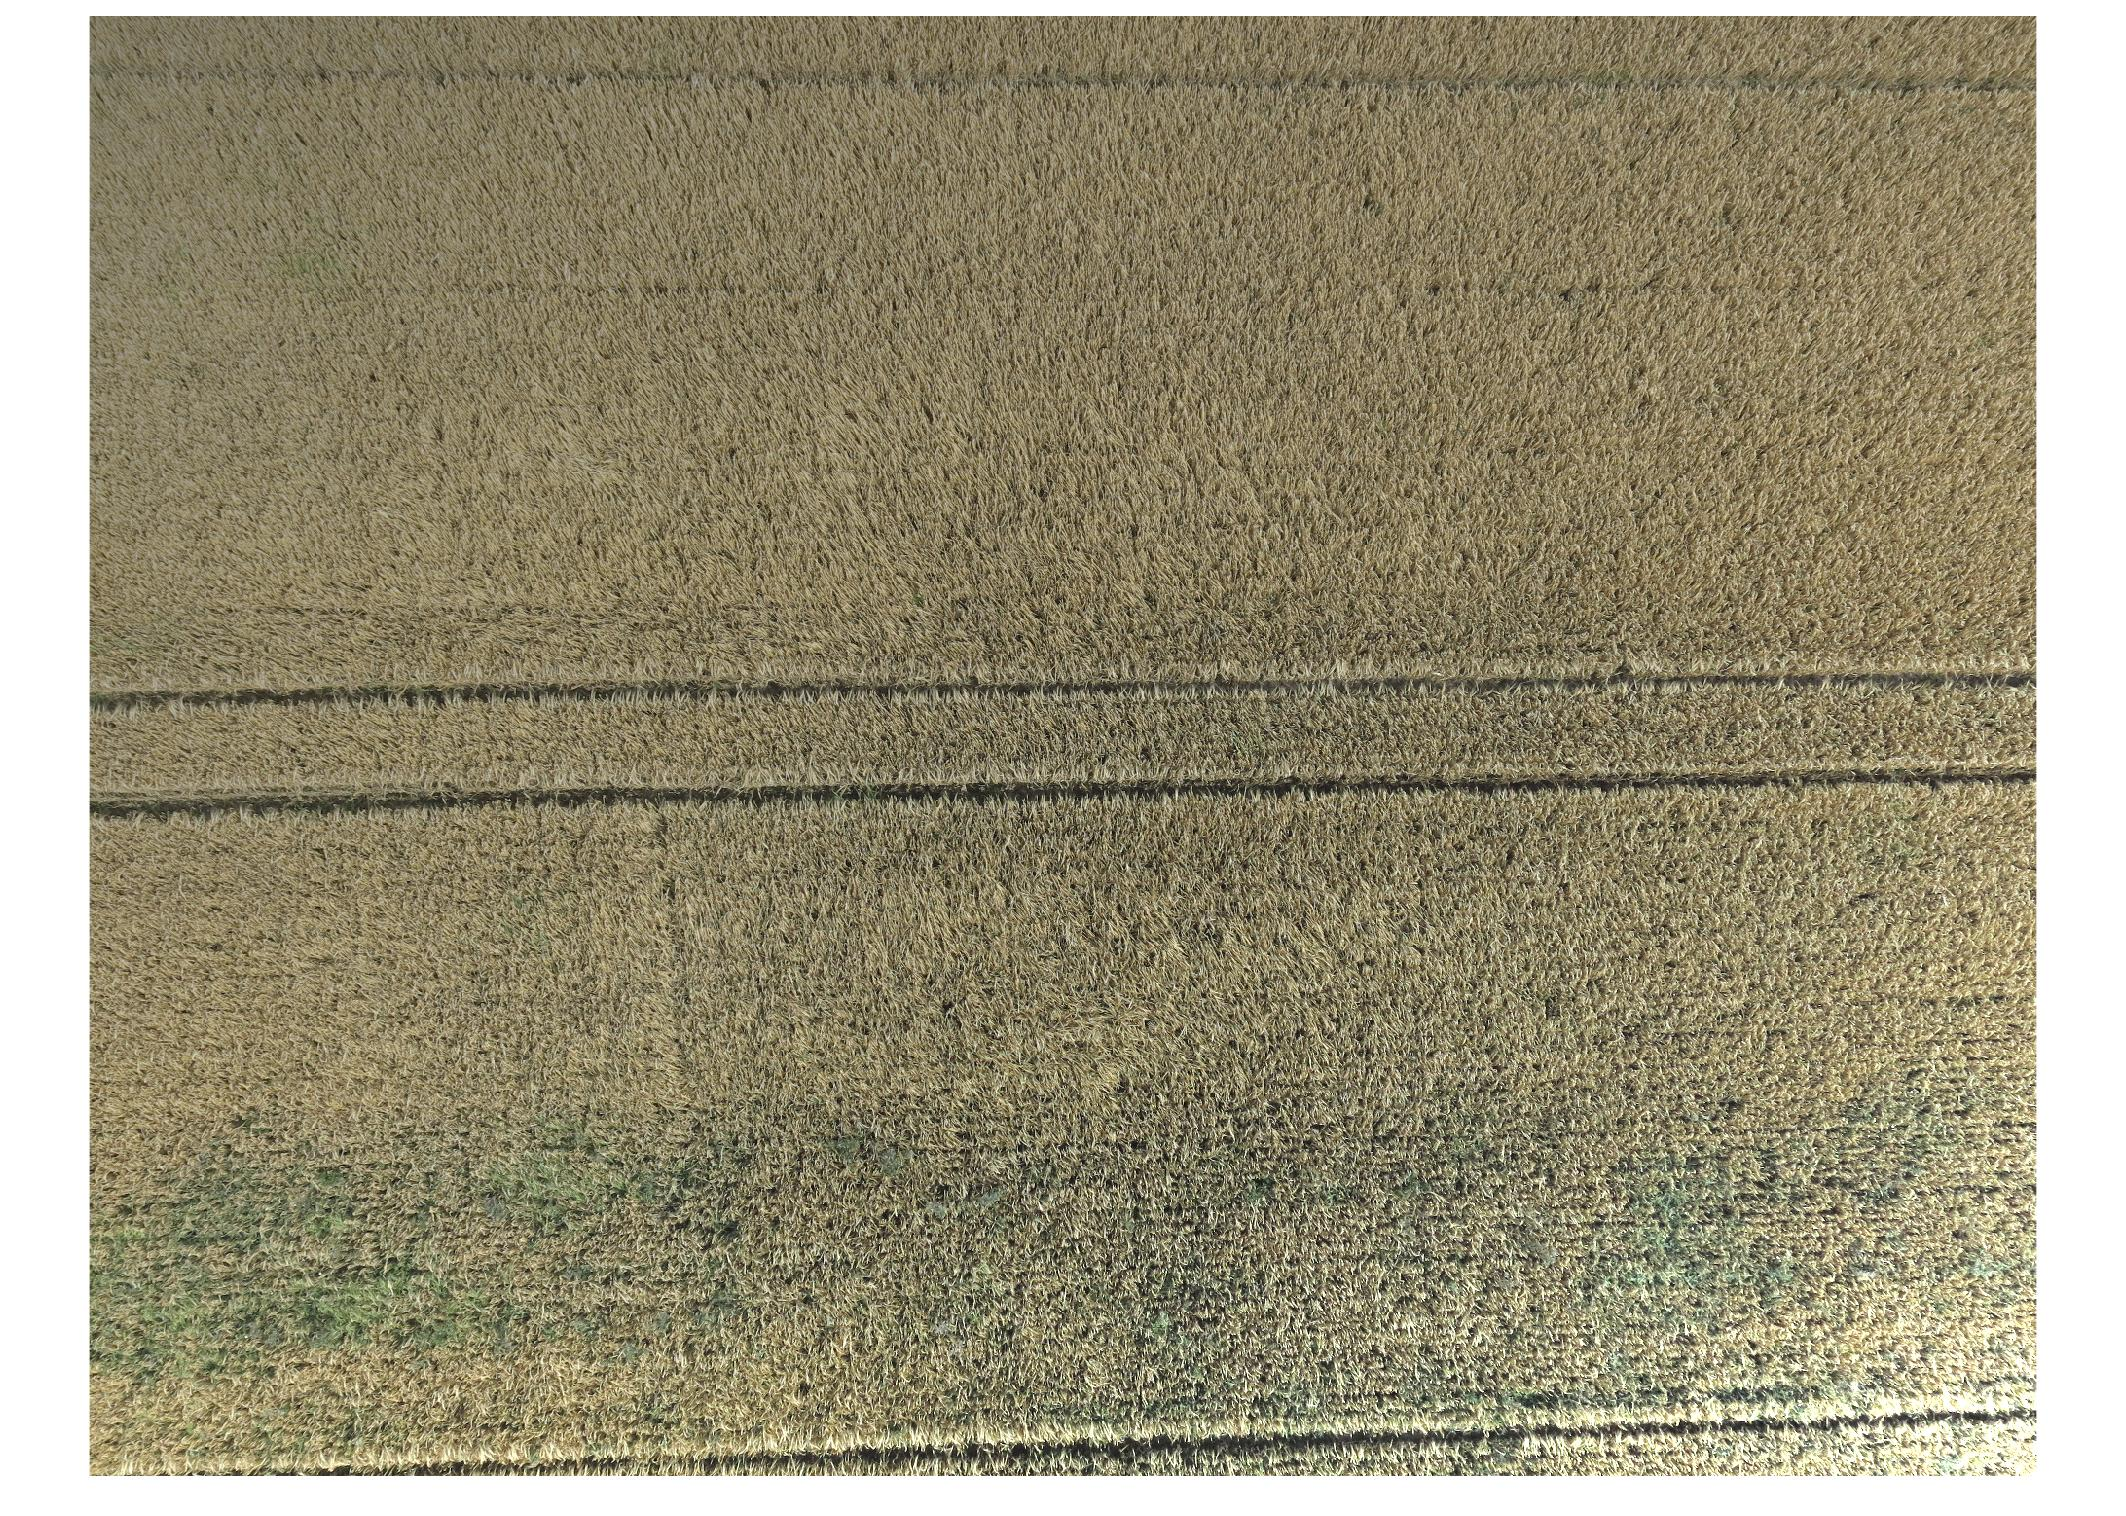
\includegraphics[width=36mm]{../IMAGES/opret0484.jpg}  
%       & \hspace{1mm} &
       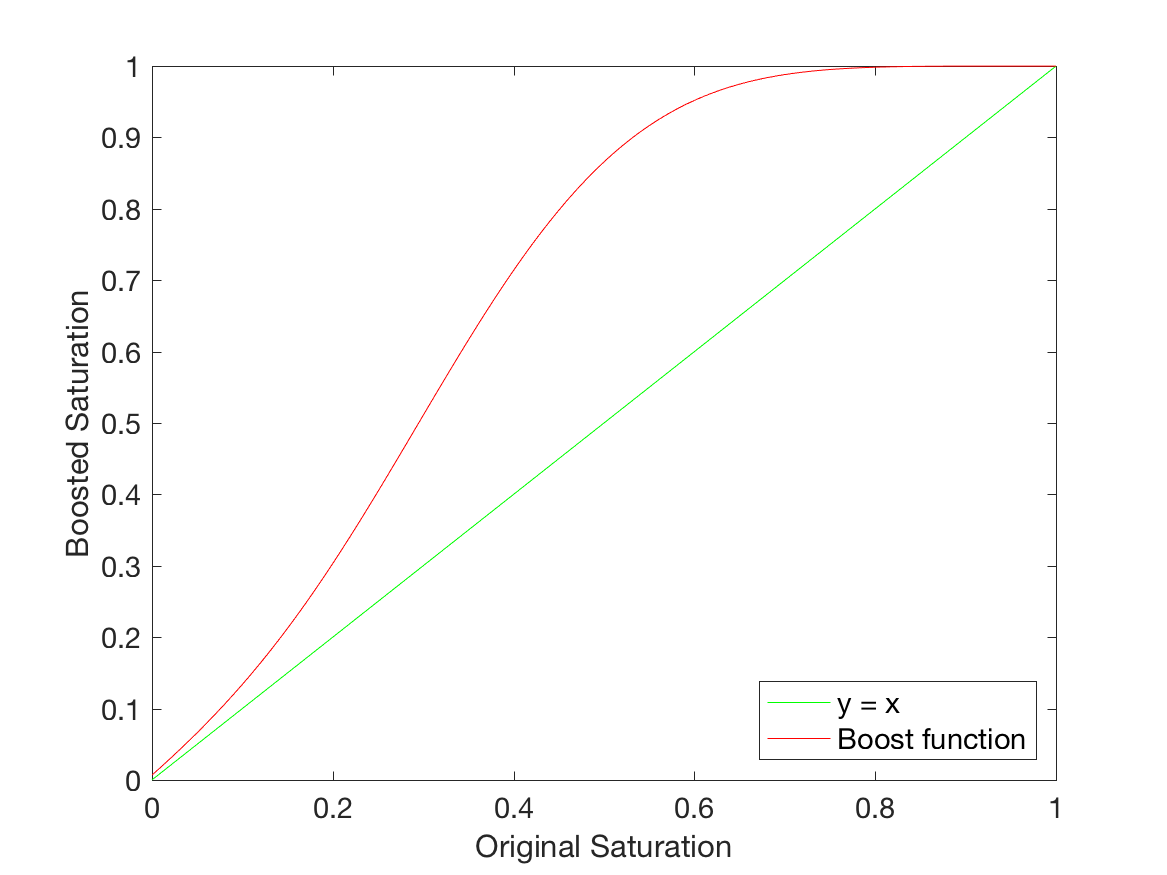
\includegraphics[width=34mm]{../IMAGES/Boostfunction.png}   
%       & \hspace{1mm} &
       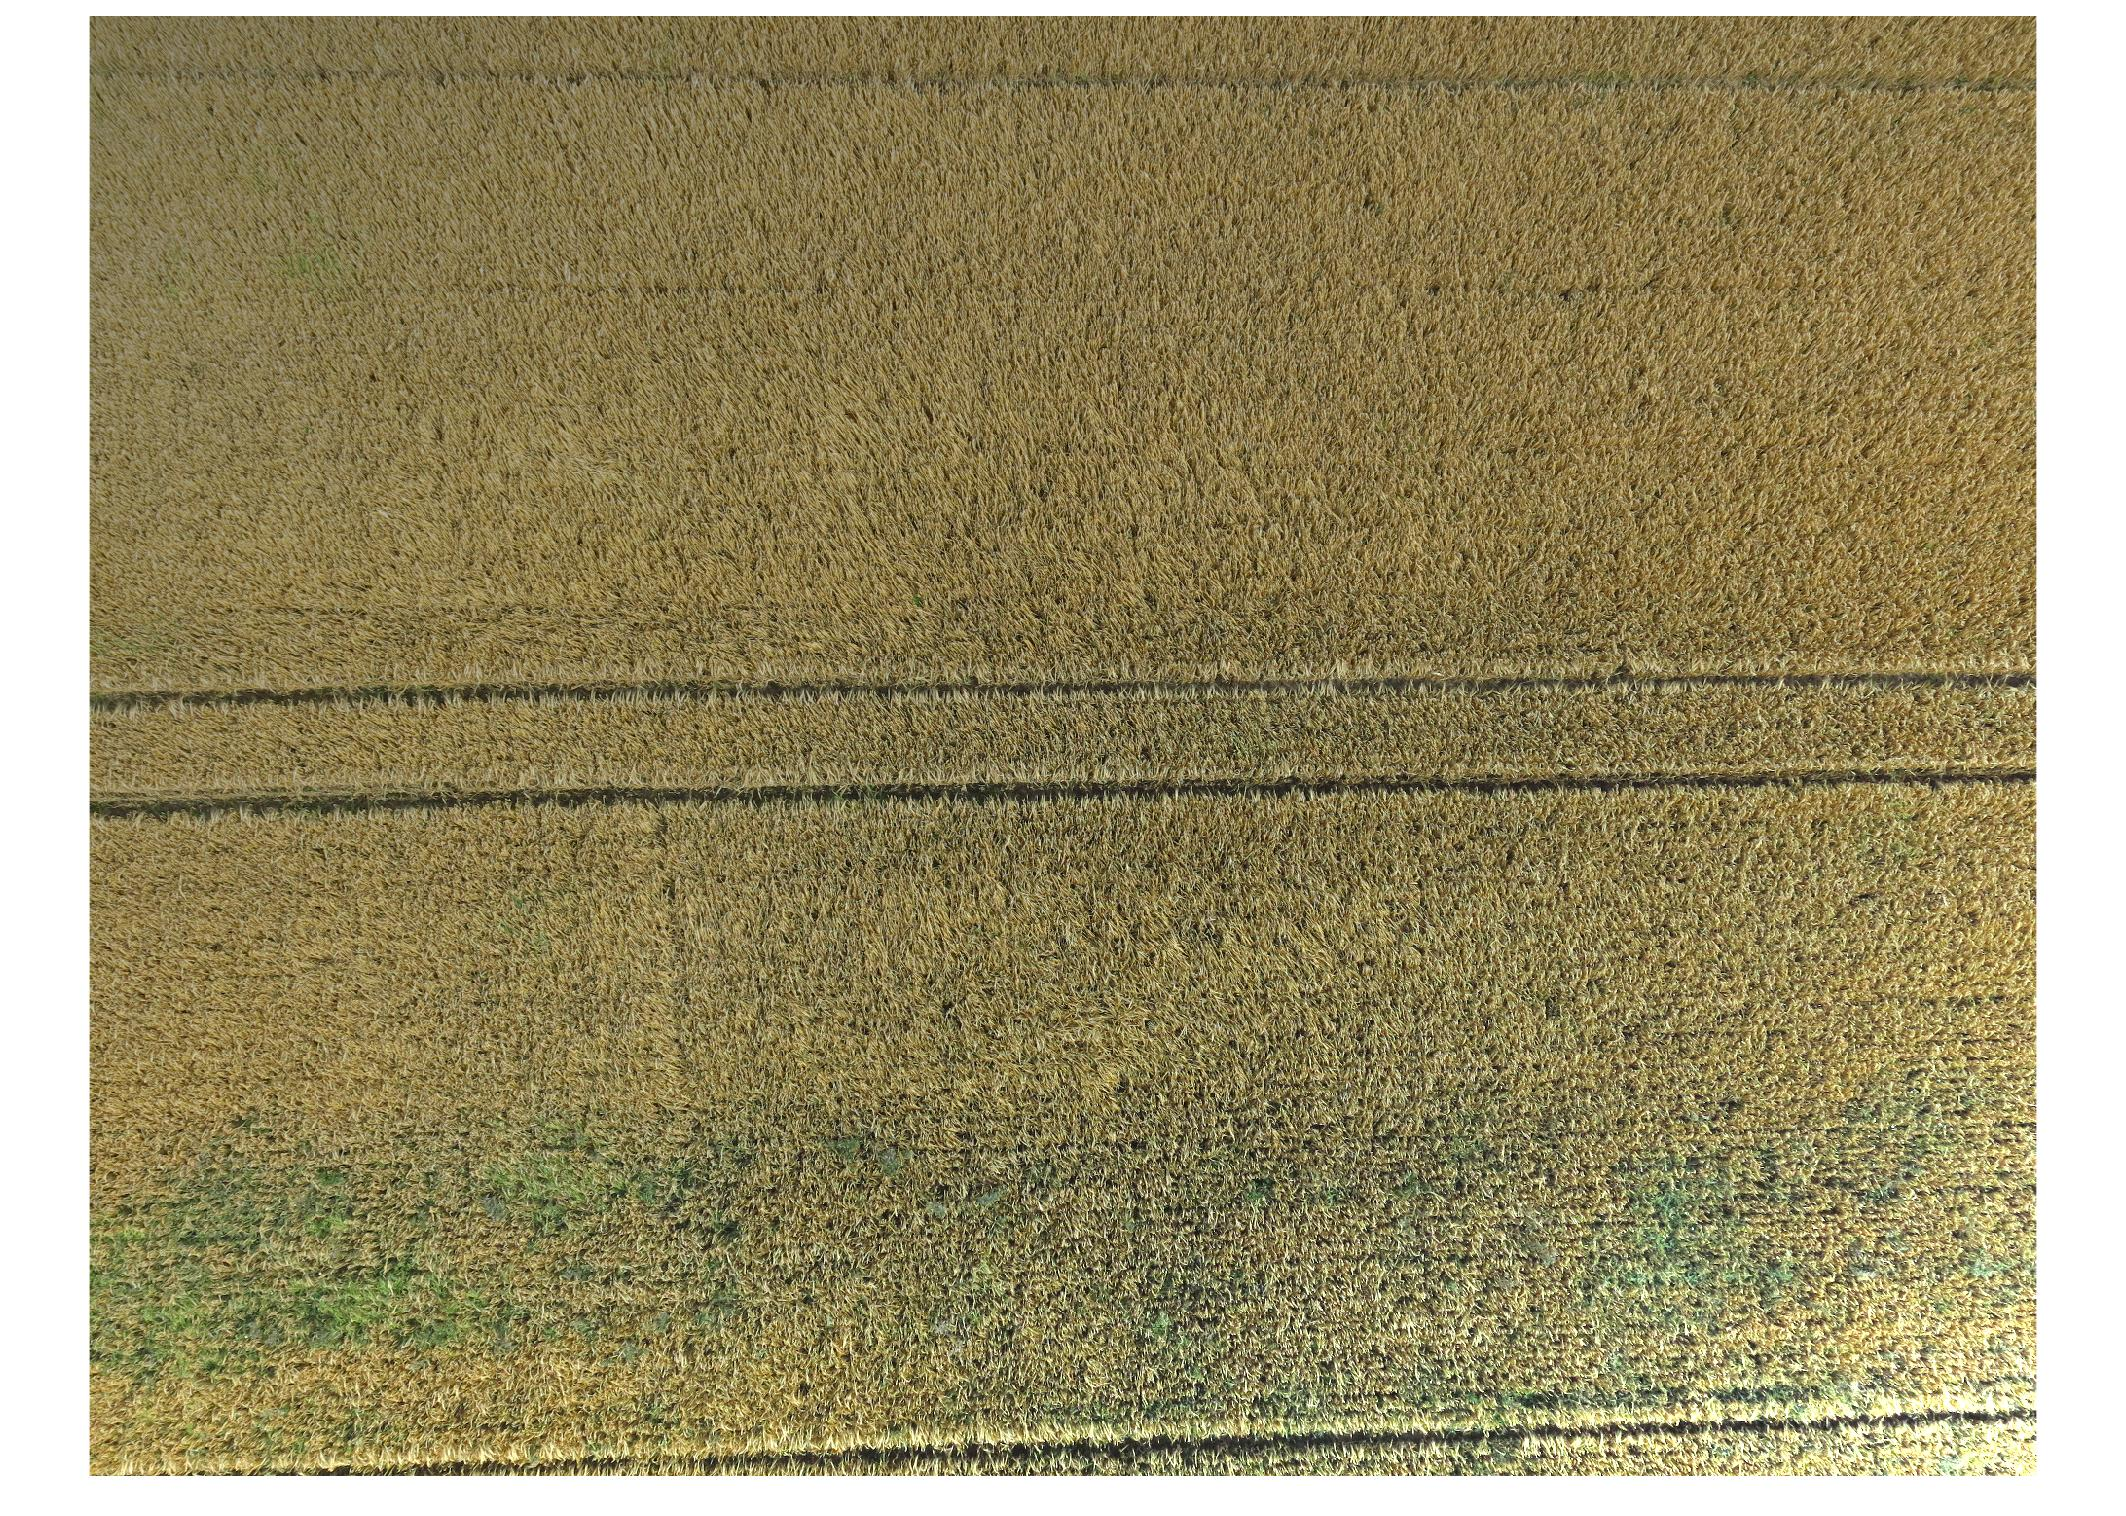
\includegraphics[width=36mm]{../IMAGES/opret2_0484.jpg} 
\end{tabular}
\end{center}


\end{frame}






%-------------------------------------------------------------------
\begin{frame} 
\frametitle{Example: Viewing the welding pool}
The light from arch welding is extremely strong and strong shielding
is needed in order to view the welding pool.

\begin{center}
\begin{tabular}{c c}
       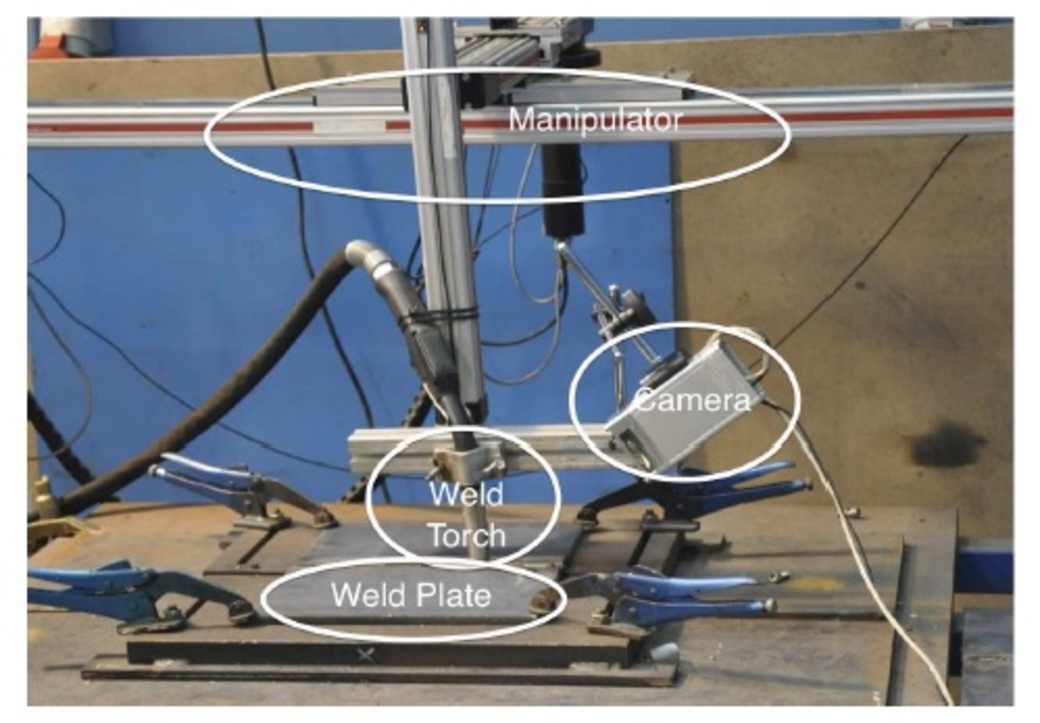
\includegraphics[width=60mm]{../IMAGES/WeldingSetUp.pdf}  
%        & \hspace{1mm} &
       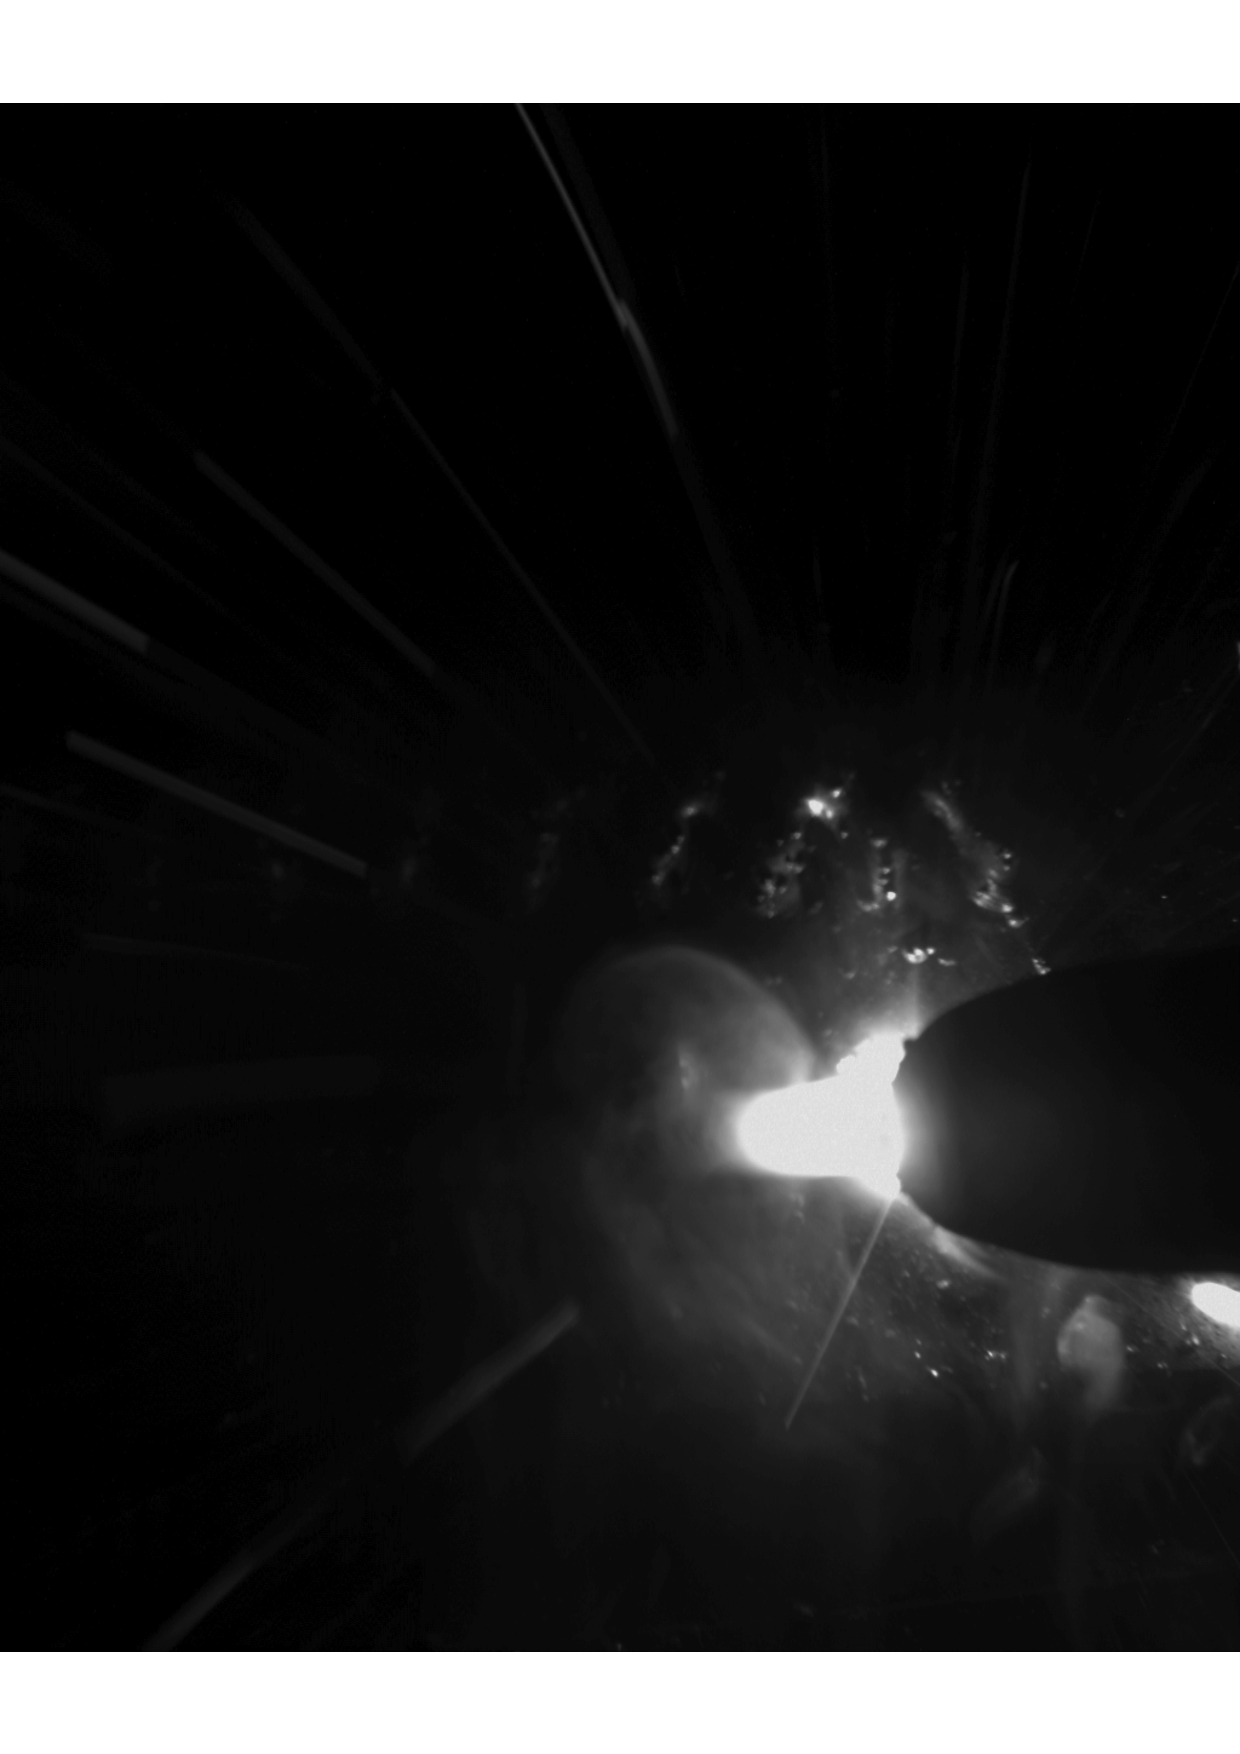
\includegraphics[width=40mm]{../IMAGES/weldpool.pdf}   
\end{tabular}
\end{center}

Work and images produces by former phD-studens Jinchao Liu
\end{frame}



%-------------------------------------------------------------------
\begin{frame} 
% \frametitle{}
In automated welding, a model of the welding pool is essential. One
approach is to select a tiny interval of the light spectrum using a
special glass that blocks all other light.

\begin{center}
\begin{tabular}{c c}
       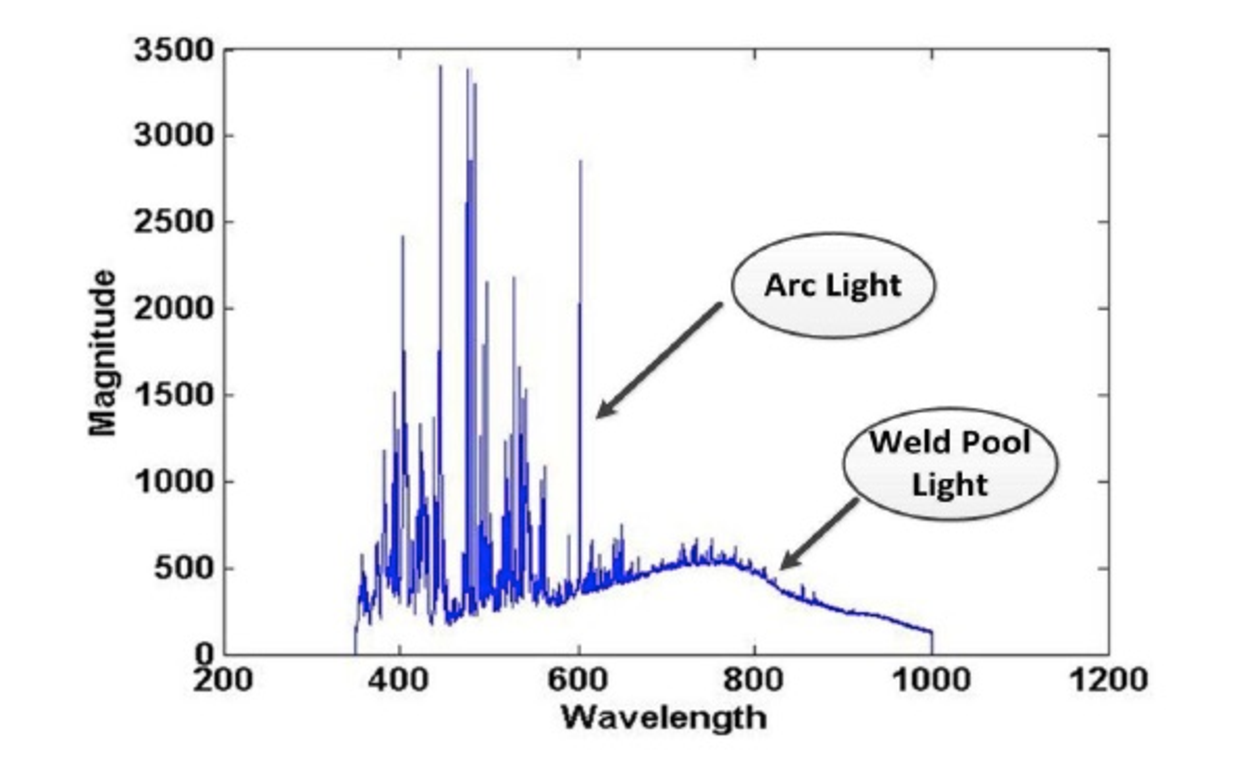
\includegraphics[width=52mm]{../IMAGES/WeldSpectrum.pdf}  
%        & \hspace{1mm} &
       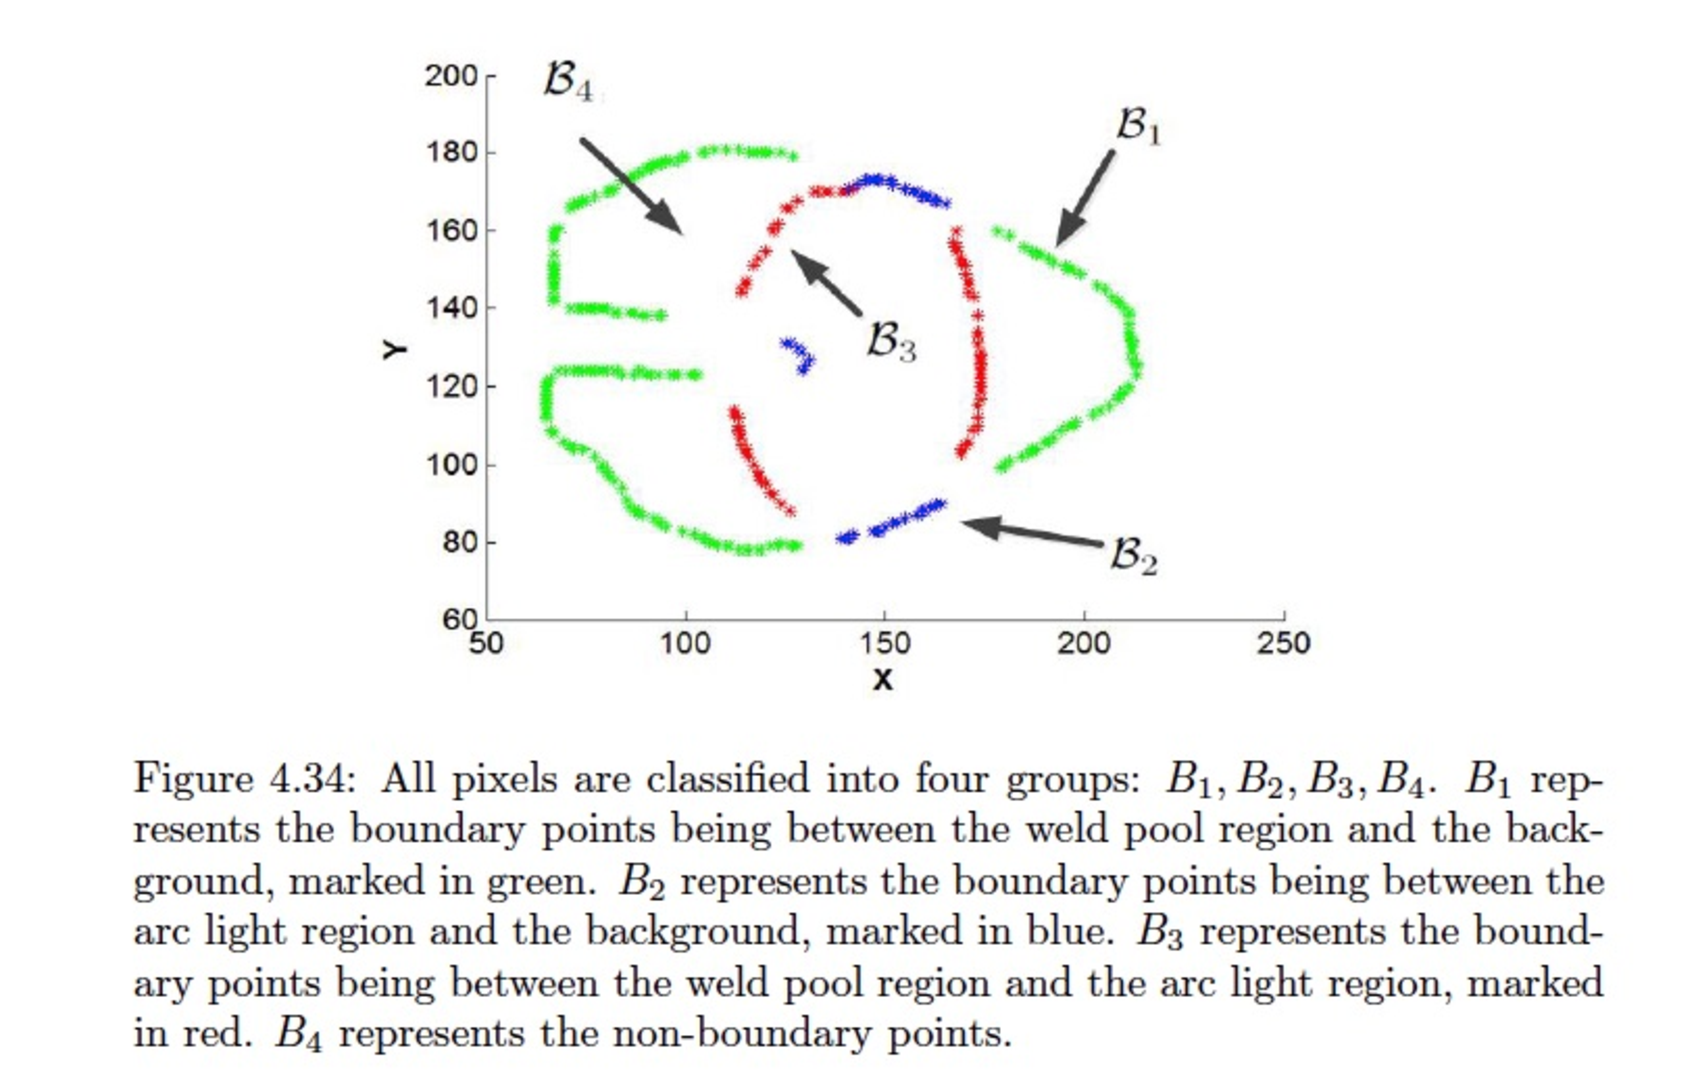
\includegraphics[width=52mm]{../IMAGES/WeldPoolModel.pdf}   
\end{tabular}
\end{center}
\end{frame}






%-------------------------------------------------------------------
\begin{frame} 
\begin{center}
       \includegraphics[width=90mm]{../IMAGES/WeldPoolImages.pdf}  
\end{center}
\end{frame}



%-------------------------------------------------------------------
\begin{frame} 
\frametitle{Example: Shadow edge removal}
Both for viewing and for object recognition it would be beneficial to
remove image edges related to shadows and leave only those related to
the objects in the scene.

\begin{center}
\begin{tabular}{c c}
       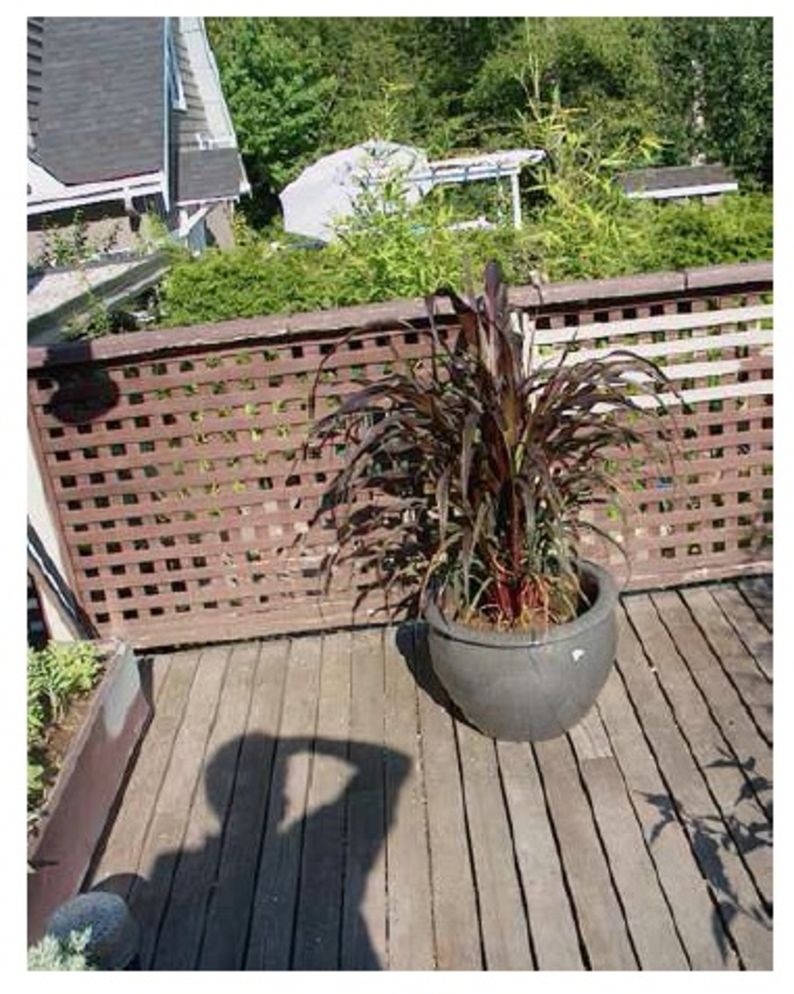
\includegraphics[width=45mm]{../IMAGES/before1.pdf}  
%        & \hspace{1mm} &
       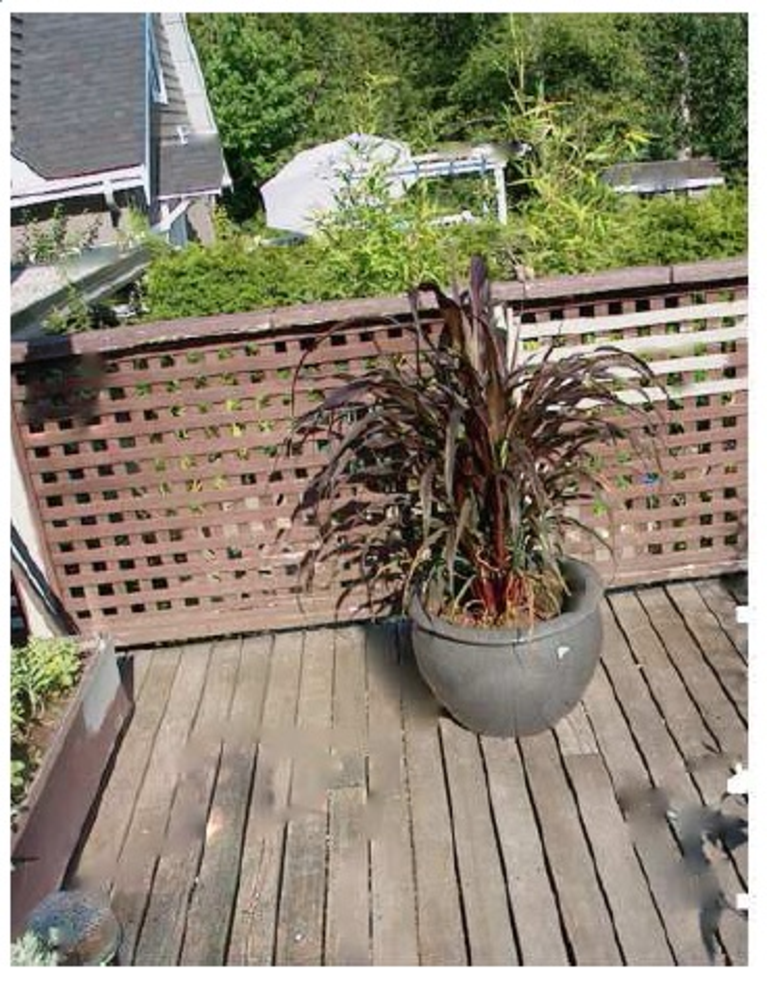
\includegraphics[width=44mm]{../IMAGES/after1.pdf}   
\end{tabular}
\end{center}
{\small 
Method and images from {\em Finlayson, Drew, lu: Entropy Minimization
  for Shadow removal}, 2007.
}
\end{frame}



%-------------------------------------------------------------------
\begin{frame} 
\frametitle{Procedure for removal}
\begin{enumerate}
\item Compute image gradients and detect edges in the image.
\item Classify the edges as shadow edges or not.
\item Remove the shadow edges by nulling the gradient information
  in a band along the shadow edges.
\item Reintegrate the gradient information and add mean color to get an
  image without shadows.
\end{enumerate}
\bigskip

The first and third steps are easy. The last step requires advanced
numerical integration routines, but is doable (we will not deal with
this step).  The challenging step is the classification. \\[3mm]

The basic idea is to transform the image into another (grey) one where 
the intensity dependency of the illumination source is canceled. Thus,
shadow edges will not exist. 
\end{frame}




%-------------------------------------------------------------------
\begin{frame} 
\frametitle{Simplification}
Remember relation between temperature of black body and emitted energy:
\begin{displaymath}
  E(\lambda) \;=\; C \frac{1}{\lambda^5} \;
        \frac{1}{e^{hc / k \lambda T} -1}
\end{displaymath}
You may look op the values for $c$, $k$ and $h$ and notice typical
values of $\lambda \approx 500 nm$ and $T \approx 10^3- 10^4 K$. Then it is
easy to see that $hc \gg k \lambda T$ and that:
\begin{displaymath}
  E(\lambda) \; \approx \; C \; \frac{e^{- hc / k \lambda T}}{\lambda^5 }
\end{displaymath}
where $C$ is some constant. \\[3mm]

Remember that received energy $r_k$ of color channel $k$ is the
product of the illuminant energy, the surface albedo, the reflection
function and the sensor sensitivity profile: 
\begin{displaymath}
    r_k     =  c_k \int_{\lambda} E(\lambda) \rho(\lambda) 
                  RF(\lambda) f_k(\lambda) d\lambda
\end{displaymath}
\end{frame}



%-------------------------------------------------------------------
\begin{frame} 
\frametitle{Assumptions}
We have here assumed that the illuminant may be modeled as a black
body. We will further assume that the scene surface is diffuse (no
specularities), that the albedo $\rho(\lambda)$ is constant as a
function of spatial coordinate and that our receptor sensitivity
profiles $f_k$ respond only to a single wavelength:

\begin{displaymath}
f_k(\lambda) \; = \; \delta (\lambda - \lambda_k) \; = \;
          \left \{
            \begin{array}{l l}
              1 & \mbox{if $\lambda = \lambda_k$} \\
              0 & \mbox{otherwise}
             \end{array}
           \right.
\end{displaymath}
We will also assume that the reflection function $RF$ is
constant. Thus:
\begin{displaymath}
    r_k    \; = \; c_k \int_{\lambda} E(\lambda) \rho(\lambda) 
                  RF(\lambda) f_k(\lambda) d\lambda
             \; = \; K \rho (\lambda_k) RF( \lambda_k)
                     \frac{e^{- hc / k \lambda_k T}}{\lambda_k^5} 
\end{displaymath}
where $K$ is a new constant and where $k \in \left \{ R,G,B \right \}$.
\end{frame}






%-------------------------------------------------------------------
\begin{frame} 
% \frametitle{}
Now let $c_1 = \log ( r_R / r_B )$ and $c_2 = \log ( r_G / r_B )$. \\

\begin{eqnarray*}
  c_1 & = &  \log \left (
             \frac{K \rho (\lambda_R) RF( \lambda_R)
                     \frac{e^{- hc / k \lambda_R T}}{\lambda_R^5}} 
                   {K \rho (\lambda_B) RF( \lambda_B)
                     \frac{e^{- hc / k \lambda_B T}}{\lambda_B^5}} 
                 \right ) \\
        & = & a_1 + \frac{1}{T} b_1
\end{eqnarray*}

where $b_1 = \frac{h c}{k} ( \frac{1}{\lambda_B} - \frac{1}{\lambda_R})$ \\[2mm]
is a constant only depending on the wavelengths and where $a_1$ is a
constant depending on $\lambda_R$ and  $\lambda_B$ and on the 
$\rho$- and $RF$ values of these.\\[3mm] 

Similarly $c_2 = a_2 + \frac{1}{T} b_2$.  Thus, when the light source
radiation, i.e. $T$ is changing, then $(c_1, c_2)$ is moving on a
straight line. Notice that $b_1$ and $b_2$ do not depend on the scene,
but only the sensors. Thus, {\color{blue}{\bf all such lines are parallel}}.
The orientation is called {\bf color temperature direction}.
\end{frame}



%-------------------------------------------------------------------
\begin{frame} 
\frametitle{The color temperature direction}

\begin{center}
       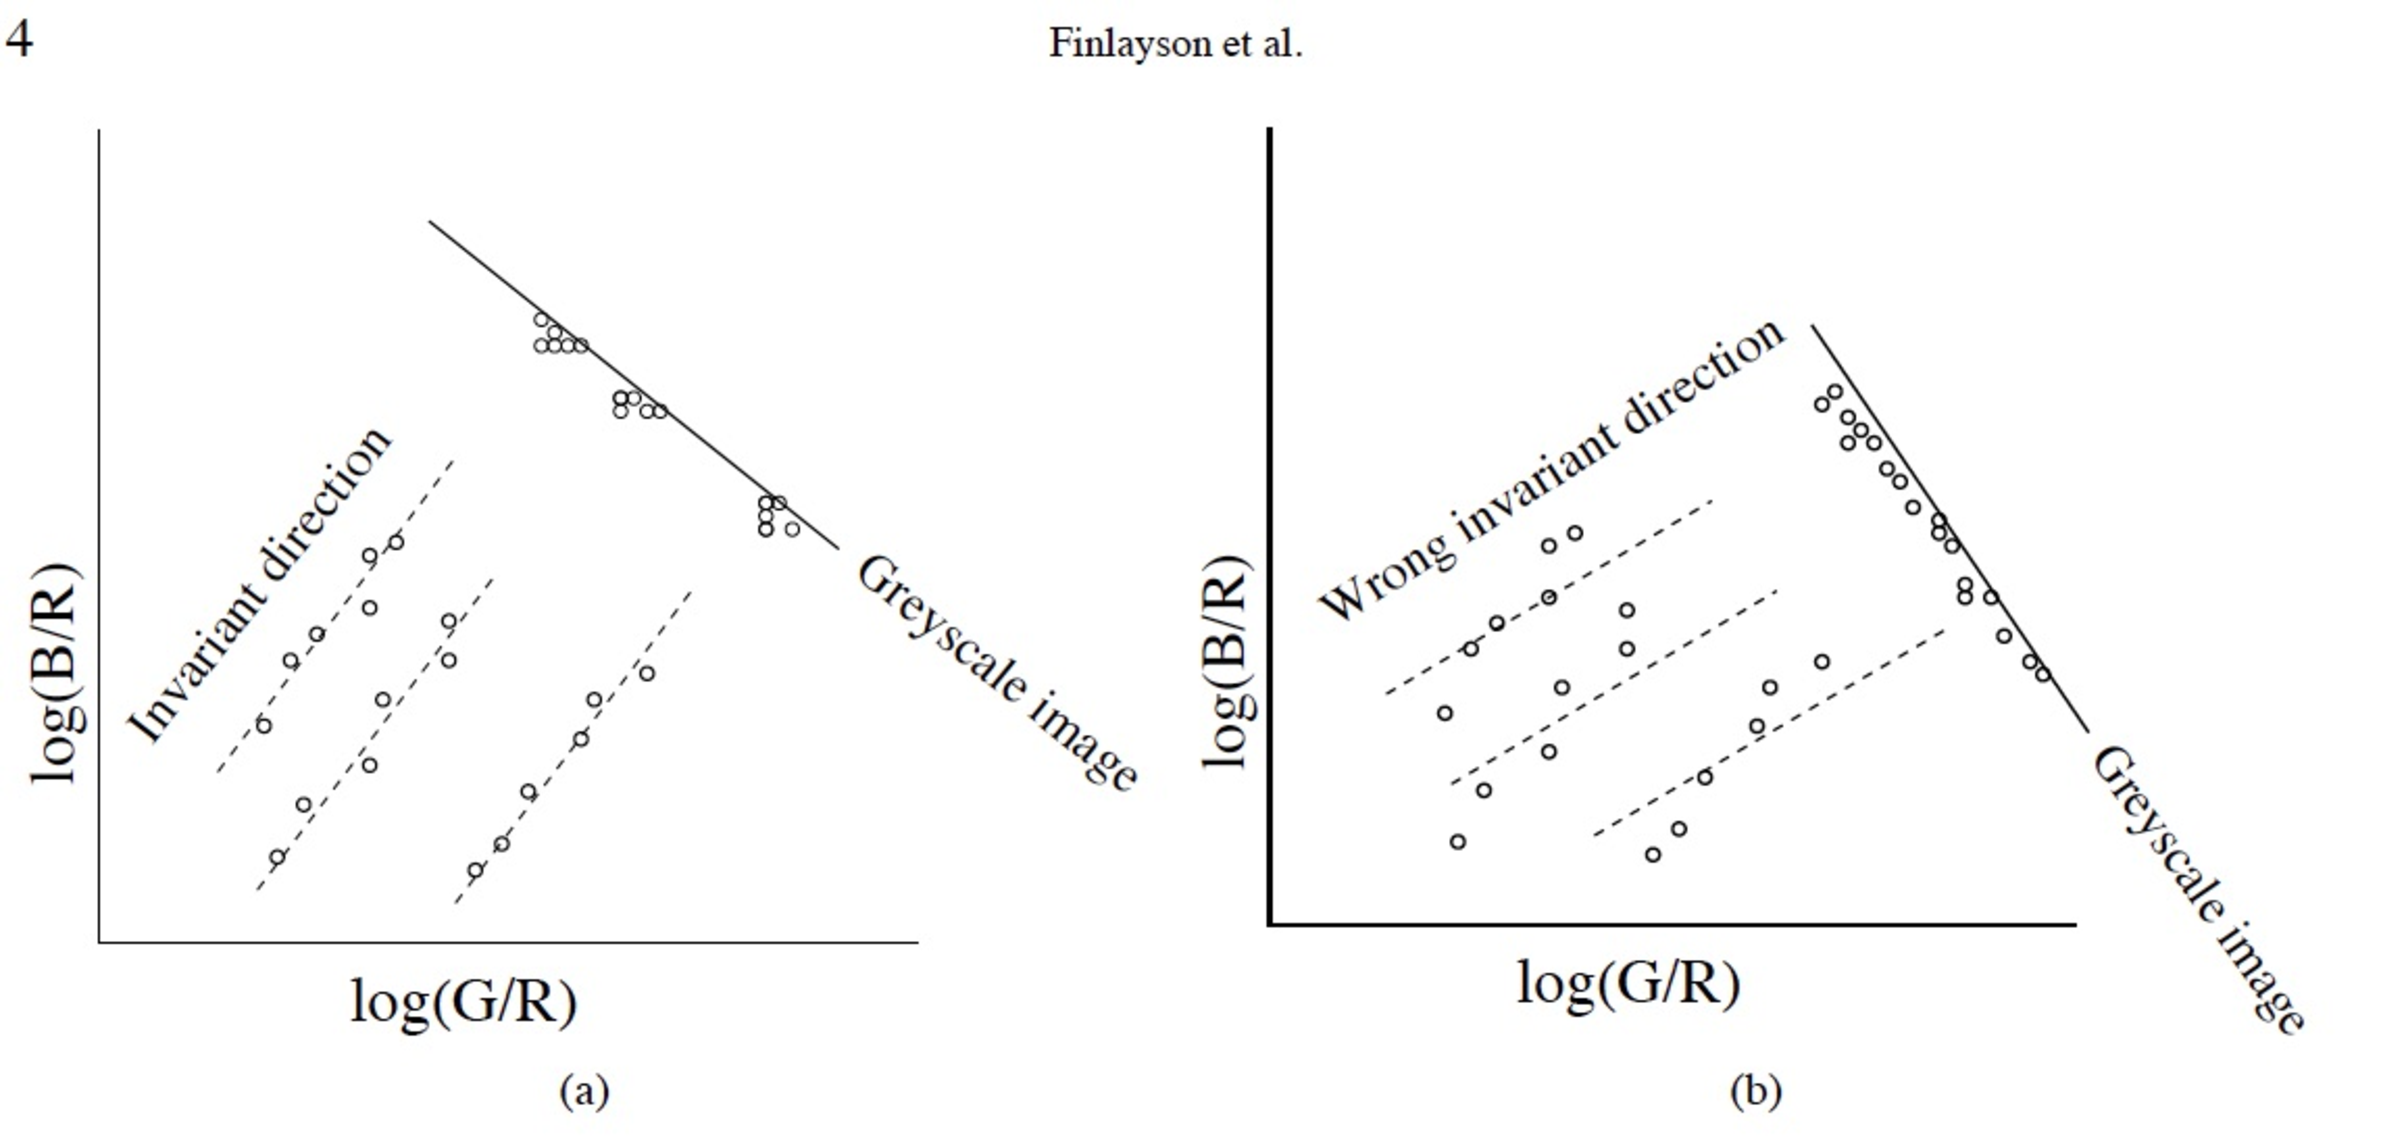
\includegraphics[width=90mm]{../IMAGES/ColorTempDir.pdf}  
\end{center}

When projecting $(c_1, c_2)$ on a line perpendicular to the color
temperature direction we will get a grey image called
{\color{blue}{The invariant image}}.  This image do not contain any
illumination effects such as shadows.
\end{frame}



%-------------------------------------------------------------------
\begin{frame} 
\frametitle{The Invariant Image}
We may compute the images $c_1 = \log (R/B)$ and $c_2 = \log (G/B)$.
If we somehow know the color temperature direction we may project the
image on a unit vector orthogonal to this.

\begin{center}
\begin{tabular}{c c}
       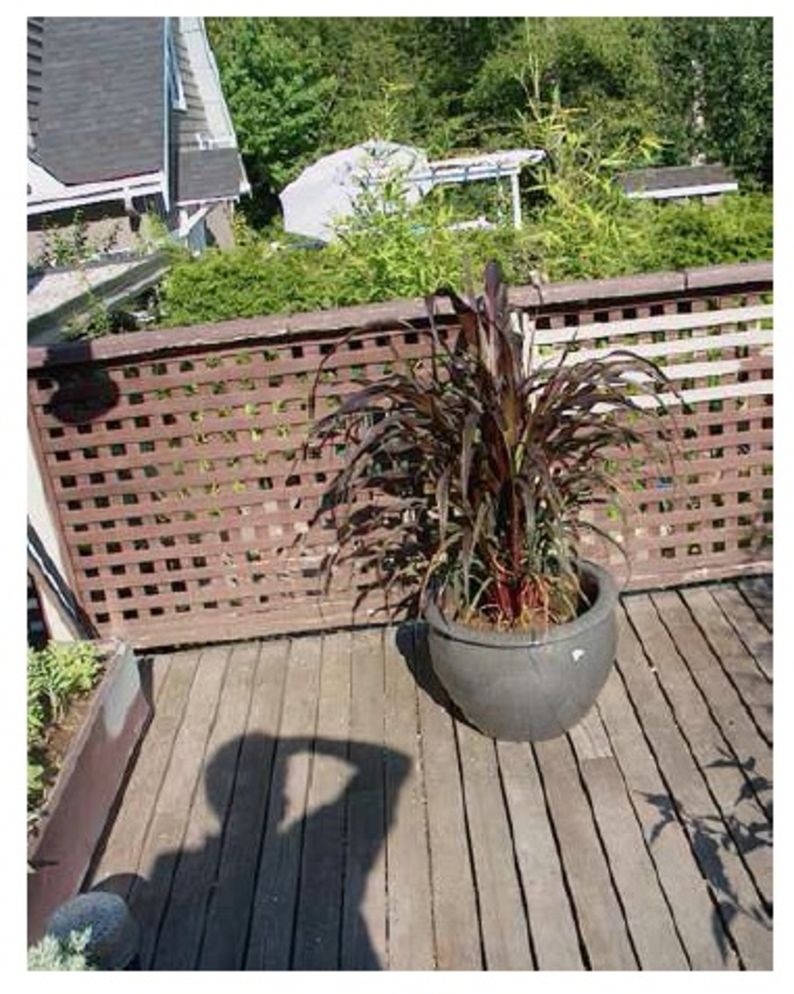
\includegraphics[width=46mm]{../IMAGES/before1.pdf}  
%        & \hspace{1mm} &
                          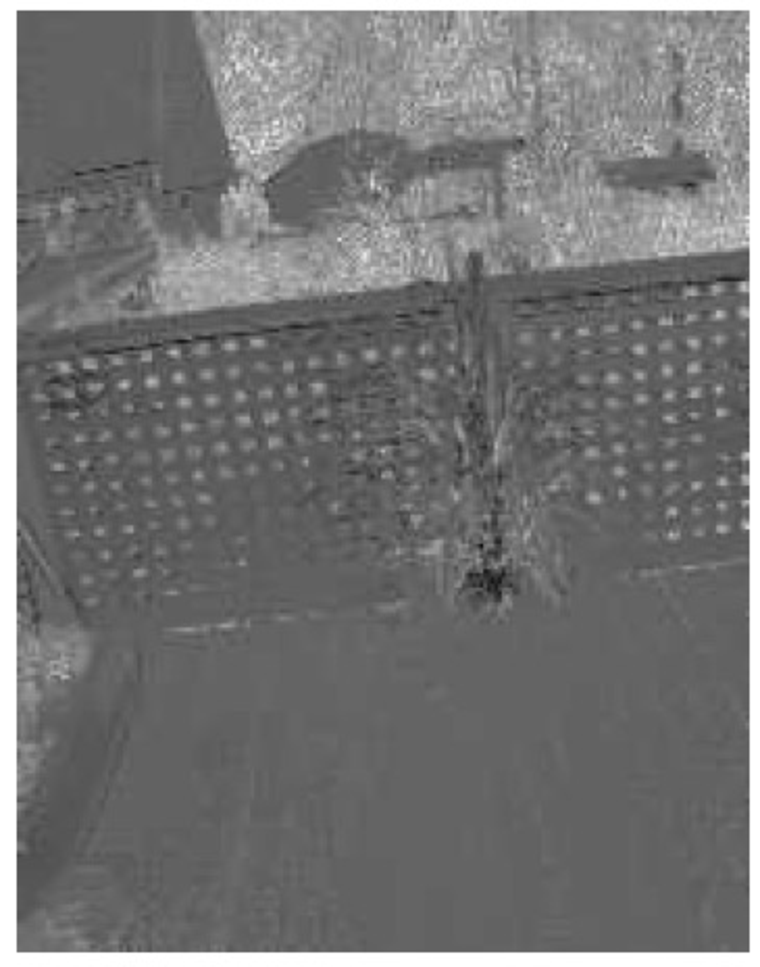
\includegraphics[width=45mm]{../IMAGES/InvariantImage1.pdf}  
\end{tabular}
\end{center}

The edges visible in the original image but not in the invariant
images may be classified as shadow edges. 
\end{frame}



%-------------------------------------------------------------------
\begin{frame} 
\frametitle{How to find the projection direction}
If many shadow edges are visible, then a lot of pixels will be arranged
along the color temperature lines in the $(c_1, c_2)$-space. Thus,
when projected on the orthogonal direction they will create a peak.
If projected on a line with any other direction they will spread more
out.

\begin{center}
       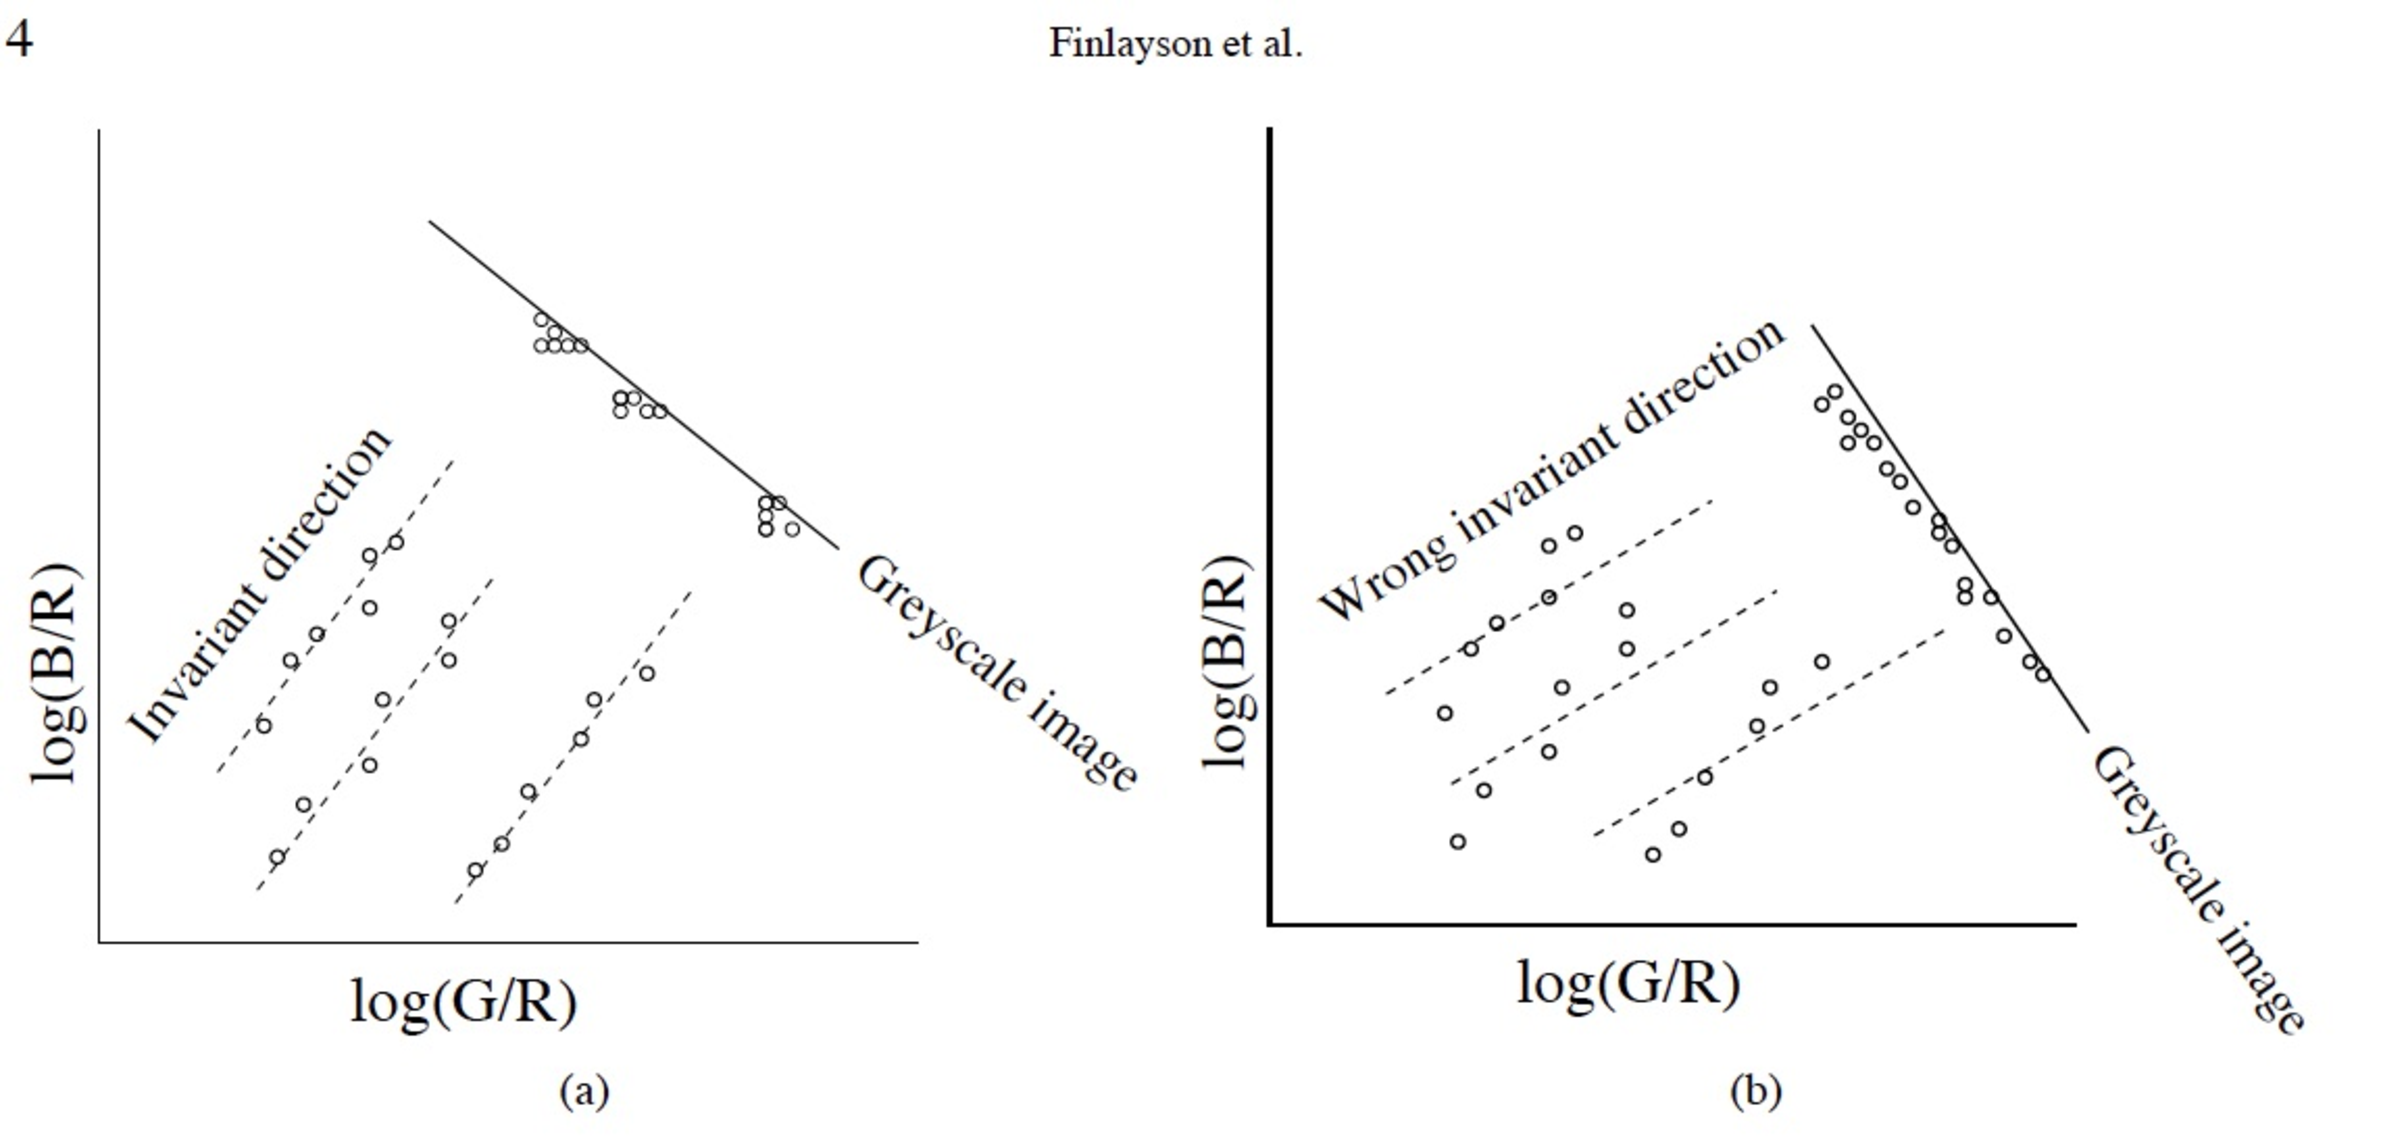
\includegraphics[width=90mm]{../IMAGES/ColorTempDir.pdf}  
\end{center}
\end{frame}



%-------------------------------------------------------------------
\begin{frame} 
\frametitle{Entropy based estimation}
The basic idea (only having access to a single image) is to project on
all possible angles ([0:180] degrees) e.g. using a quantisation of 1
degree. For each projection, i.e. a grey-valued image, we compute how
peaked the projection is, and select the one maximising this. \\[3mm]

Entropy, is a statistical measure of the spread of a probability
density distribution. Entropy is used intensively in Computer Vision
and Image Analysis to characterise distributions 

\begin{displaymath} 
  H \;=\; - \; \sum_i p_i \log p_i   
\end{displaymath}
In our case $p_i$ is the empirical probability that a pixel takes the
value $i$. \\[3mm]

In practice Finlayson et.al. do not use entropy directly, but a more
robust measure called {\em Information potential}, but this is of
minor importance.
\end{frame}



%-------------------------------------------------------------------
\begin{frame} 
\frametitle{Entropy}
Please notice that if $p$ is uniformly distributed on say 64 bins,
then $H = - 64 \frac{1}{64} \log_2 (\frac{1}{64}) = \log_2 (64) = 6$.
If $p$ is ultimately peaked (i.e. a delta-function) $H = 0$. In all
other cases $H$ is in between the two values. \\[5mm]

\begin{center}
       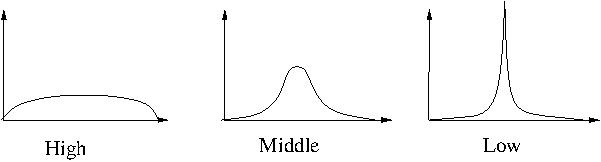
\includegraphics[width=100mm]{../FIGURES/Entropyfig.jpg}  
\end{center}



Please notice that the projection $(c_1 , c_2) \cdot (\cos v , \sin v)^{\top}$
gives an image of real values and need to be quantized when computing
a histogram of the values.  Finlayson use 64 bins. Also note that the
histogram needs to be normalized to have unit sum before entropy
computation. 
\end{frame}



%-------------------------------------------------------------------
\begin{frame} 
\frametitle{Shadow edges}
Edges visible in the original image, but not in the invariant images
are deleted by setting the partial derivatives to zero in all such
edge pixels and in the neighboring pixels up to a distance of 2
pixels. 

\begin{center}
       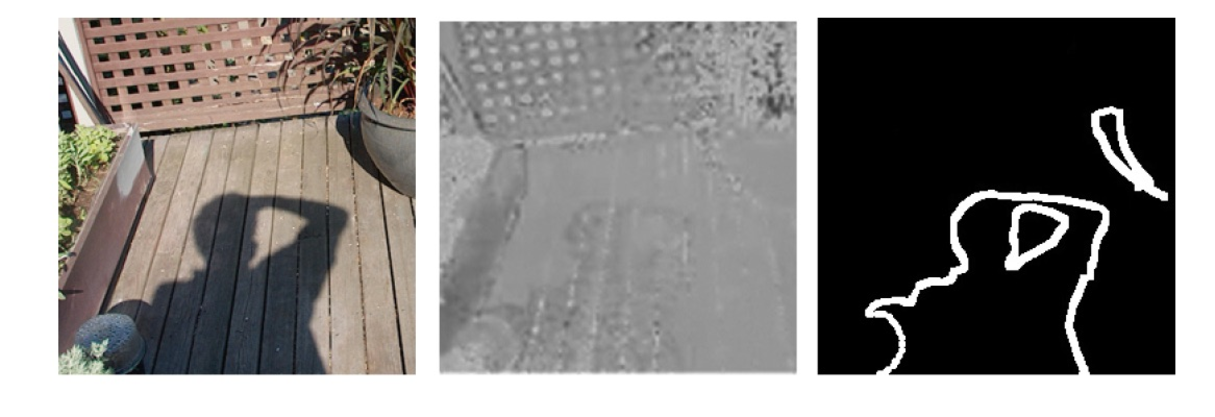
\includegraphics[width=100mm]{../IMAGES/ShadowEdges1.pdf}  
\end{center}

Before zeroing however, all detected shadow edges need to be closed in
order for the following reintegration procedure to work.  The image
border may participate in this closing.
\end{frame}



%-------------------------------------------------------------------
\begin{frame} 
\frametitle{Examples from Finlayson et.al}
\begin{center}
       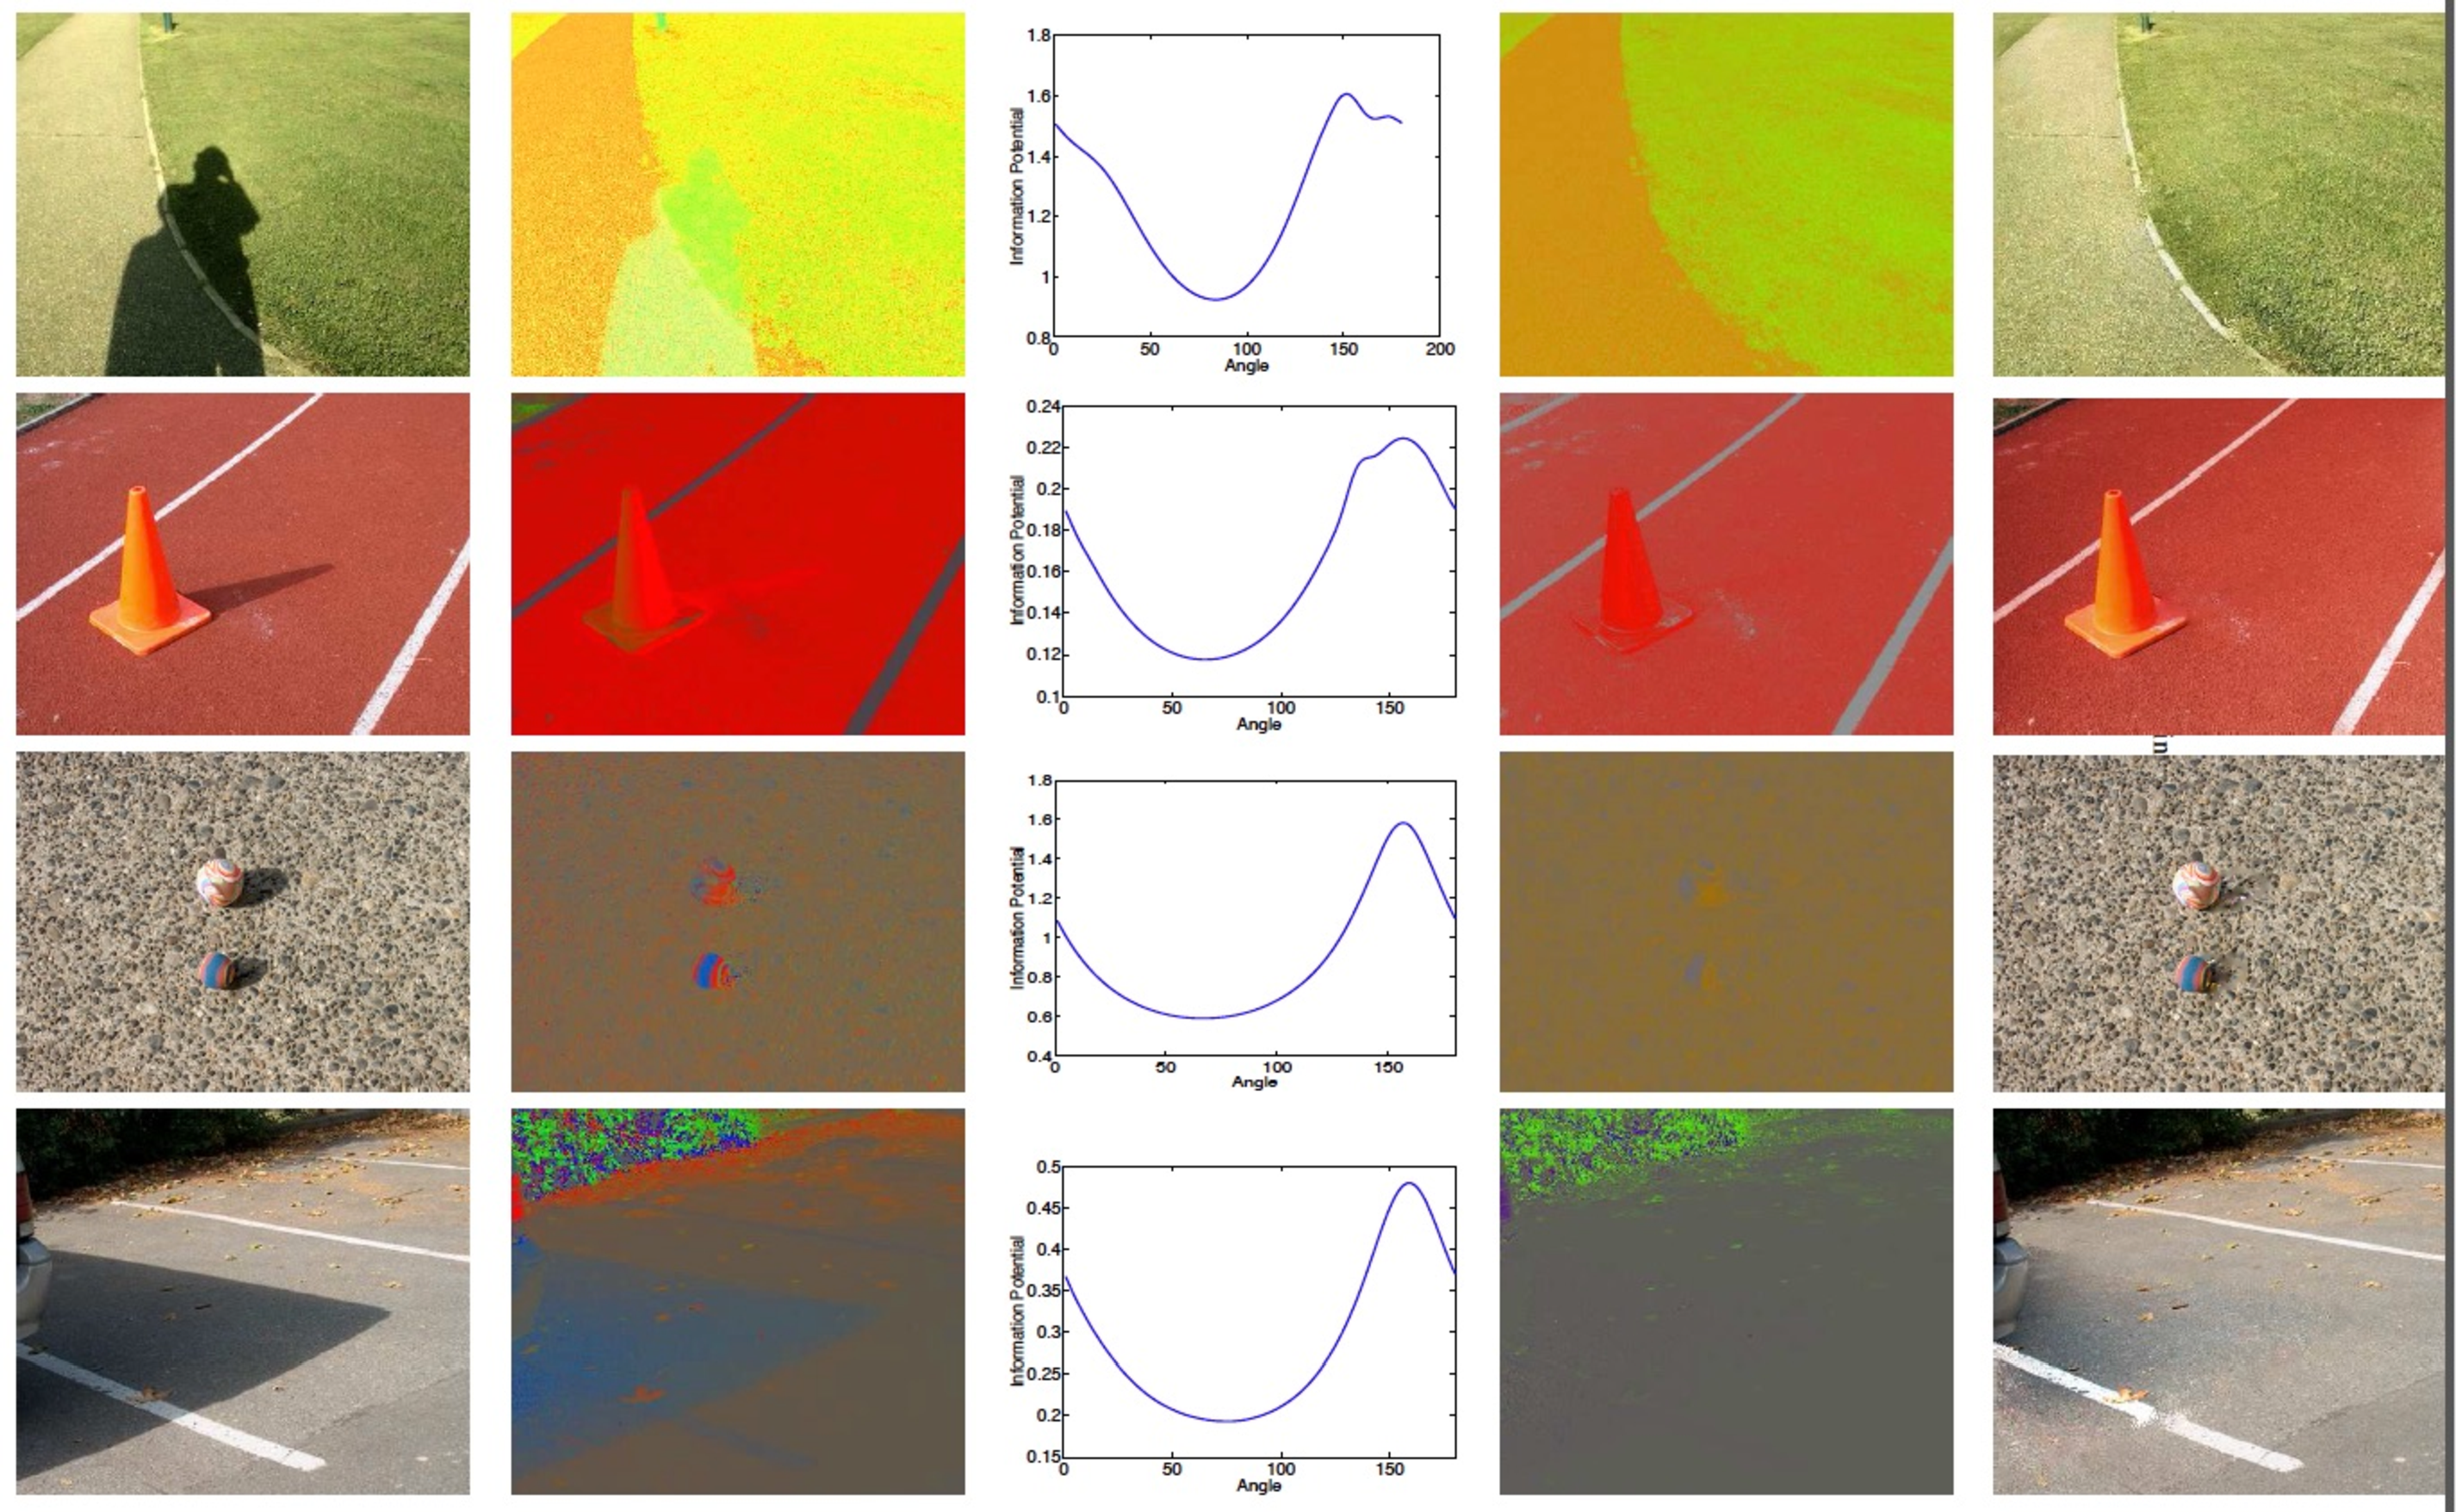
\includegraphics[width=110mm]{../IMAGES/BeforeAfter4.pdf}  
\end{center}
\end{frame}



%-------------------------------------------------------------------
\begin{frame} 
\frametitle{More examples from Finlayson et.al.}
\begin{center}
       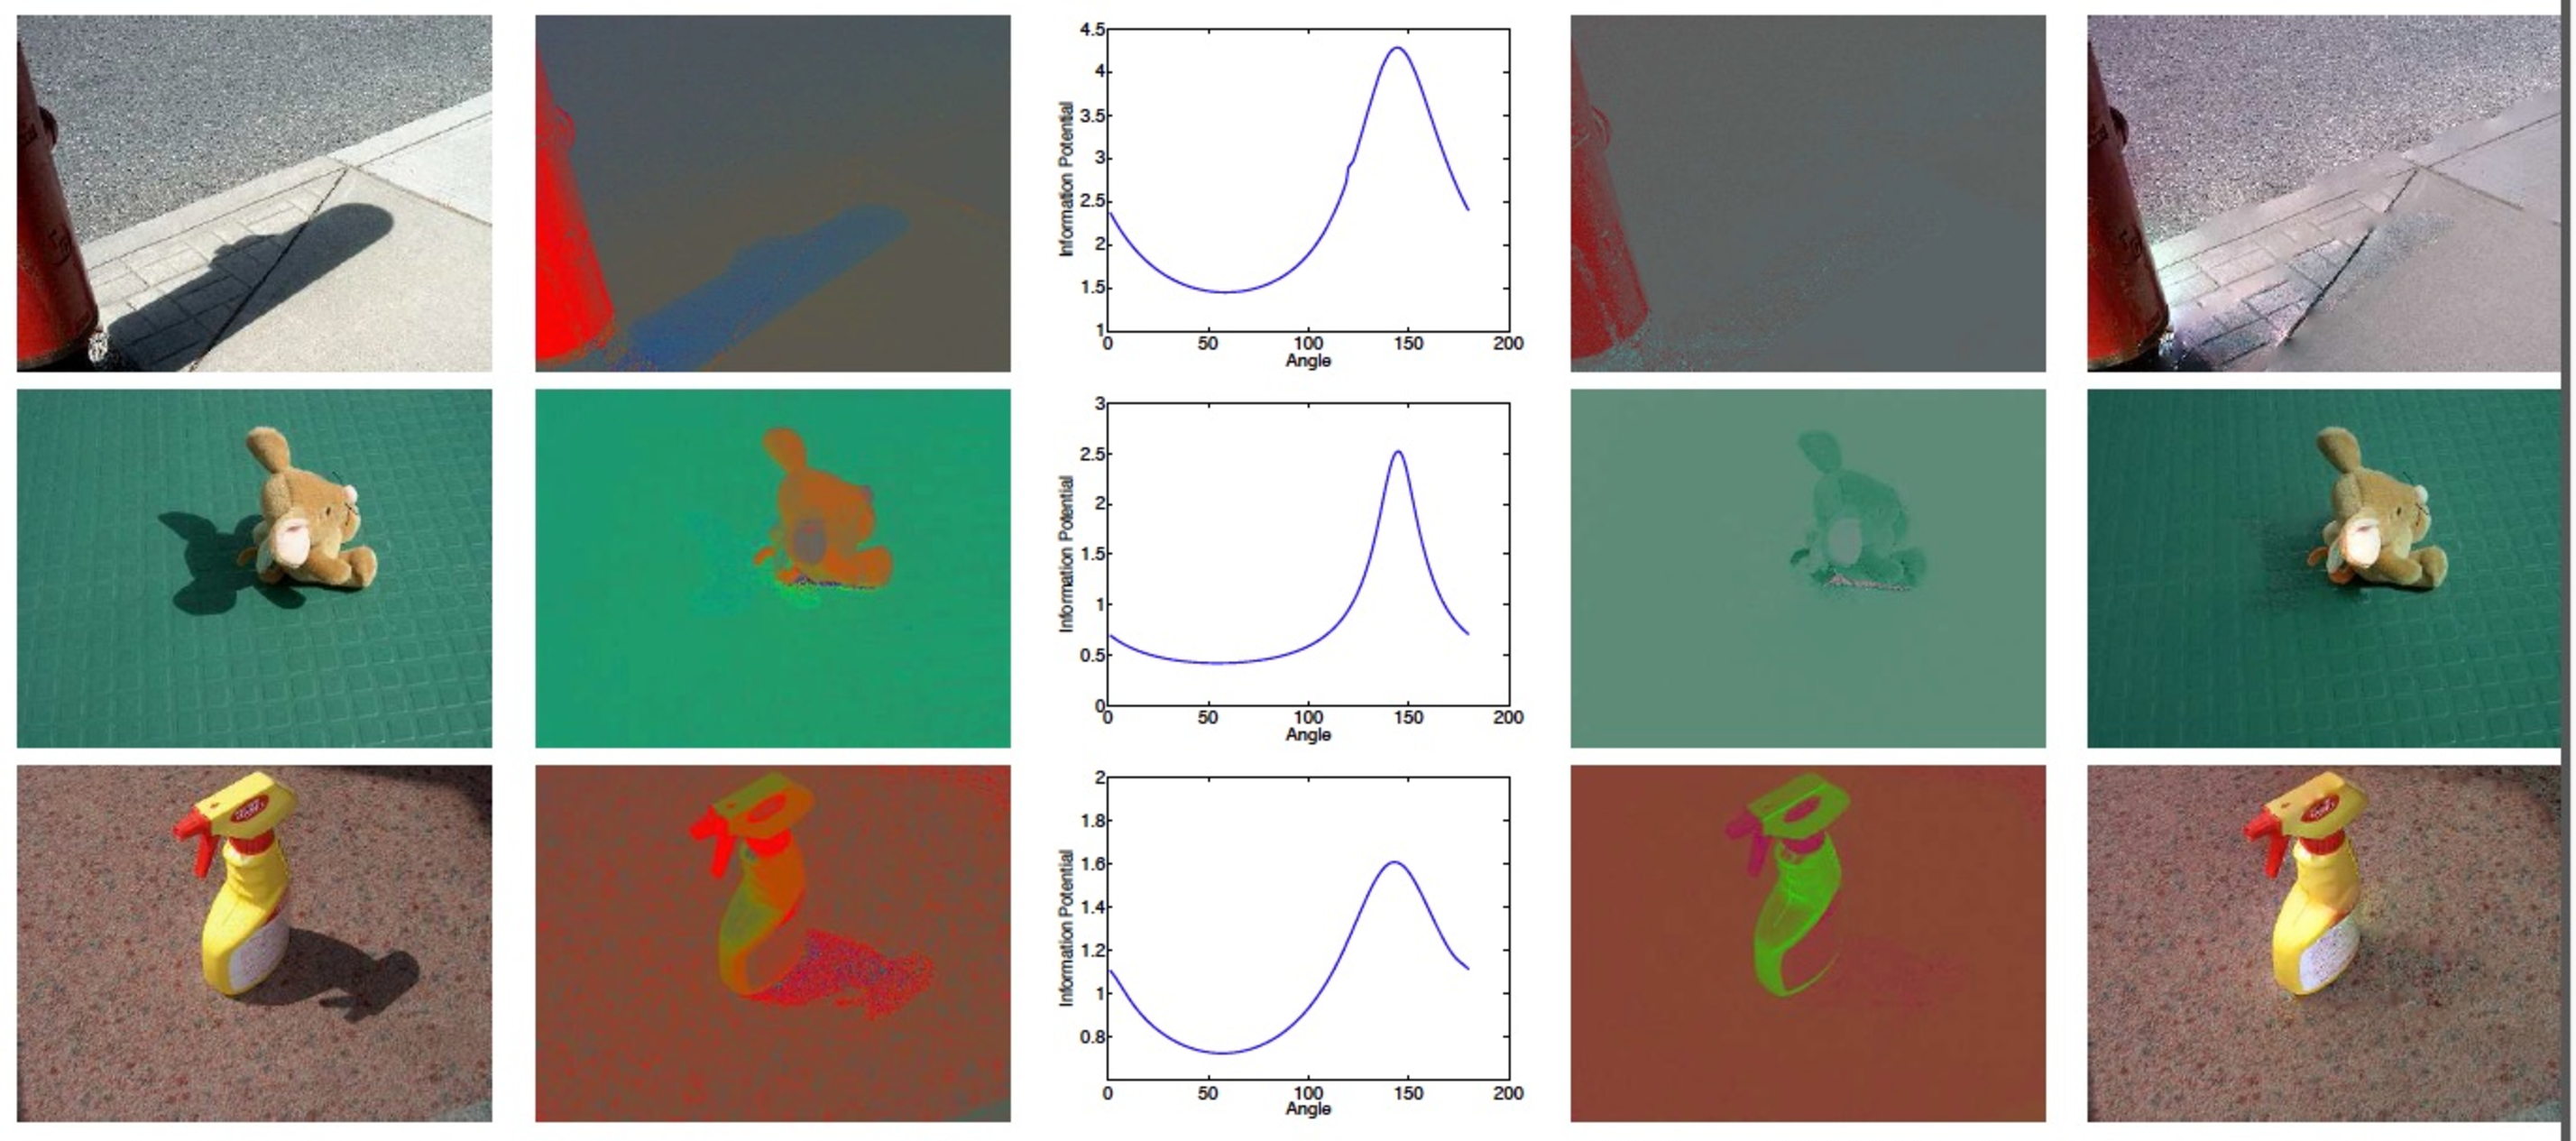
\includegraphics[width=110mm]{../IMAGES/BeforeAfter3.pdf}  
\end{center}
\end{frame}


%-------------------------------------------------------------------
\begin{frame} 
\frametitle{Examples from Fredembach et.al.}
\begin{center}
       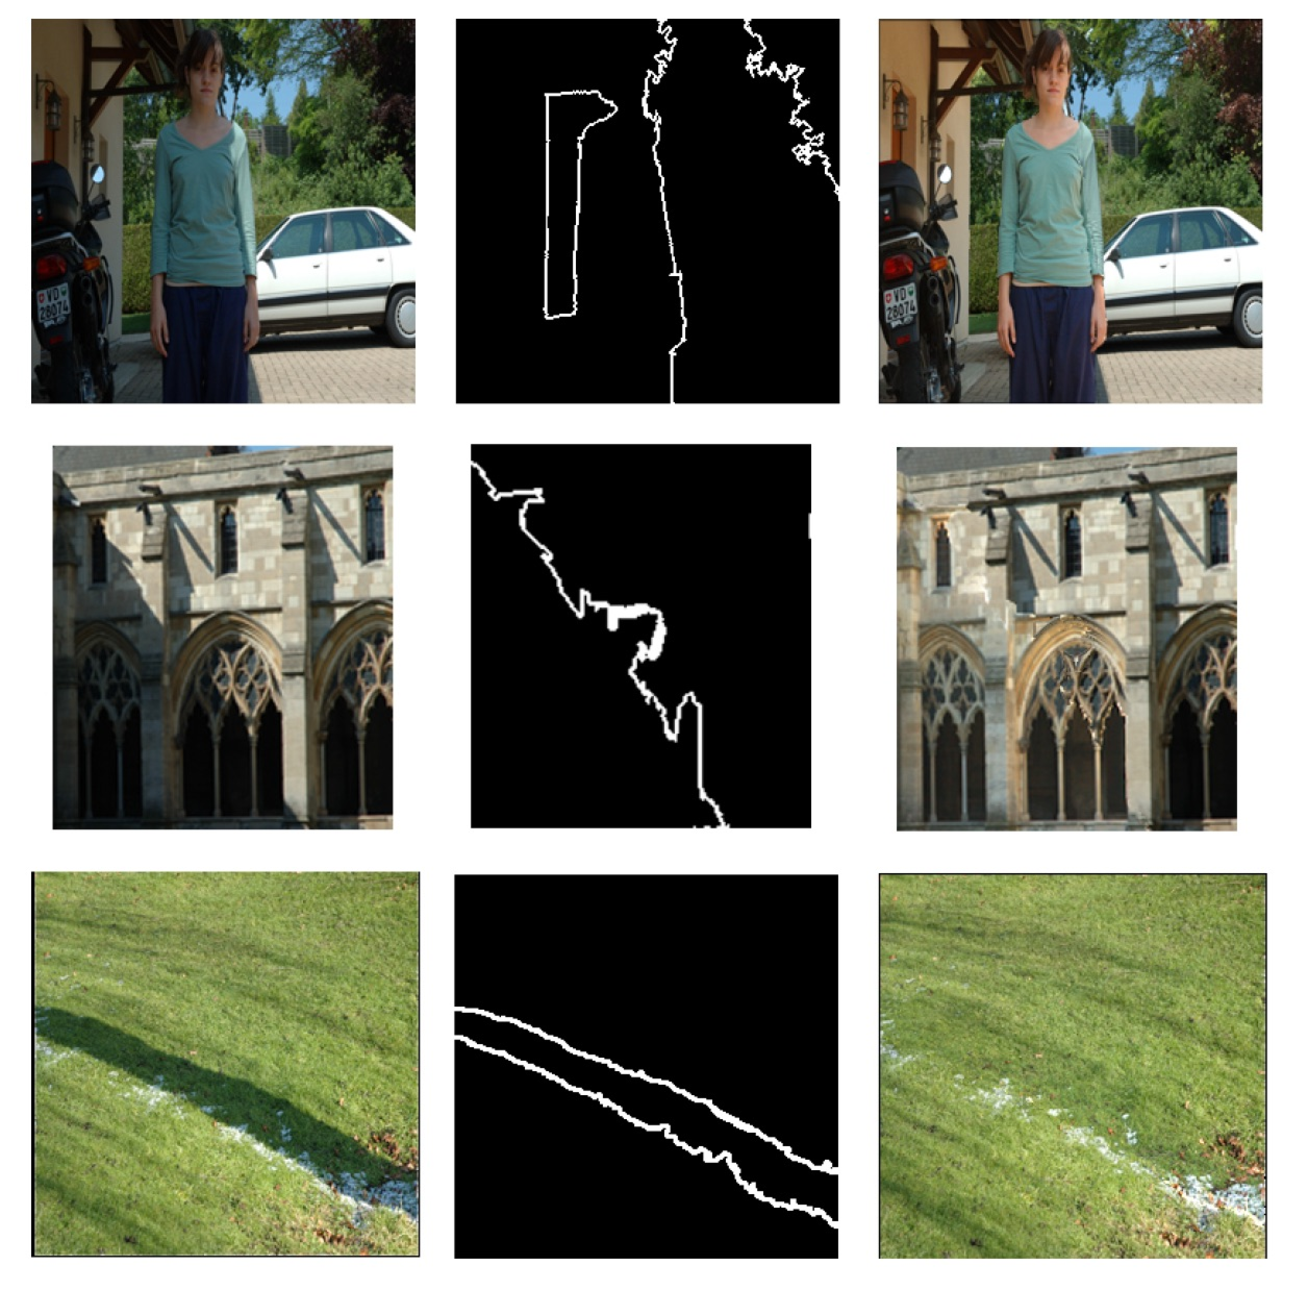
\includegraphics[width=80mm]{../IMAGES/ShadowEdges3.pdf}  
\end{center}
\end{frame}



%-------------------------------------------------------------------
\begin{frame} 
% \frametitle{Examples from Fredembach et.al.}
\begin{center}
  {\color{blue}{\Huge Questions ?}}
\end{center}
\end{frame}



%-------------------------------------------------------------------
\begin{frame}
  \frametitle{Next time}
\begin{itemize}
\item A bit on Computer Vision history
\item Neural Net basics
\item Modern Convolutional Neural Nets (CNN's)
\item Image classification, Object detction, and image segmentation
\end{itemize}
\end{frame}






\end{document}


